\documentclass[12pt,openany]{book}

\usepackage{amsmath,amssymb,amsthm}
\usepackage{graphics,epsfig,psfrag}
\usepackage{makeidx}

\topmargin          0in
\headheight         0.25in
\headsep            0.25in
\oddsidemargin      0.5in
\evensidemargin     0.5in
\textheight         8.5in
\textwidth          5.5in

\newtheorem{theorem}{Theorem}
\newtheorem{proposition}{Proposition}
\newtheorem{definition}{Definition}
\newtheorem{example}{Example}

\newcommand{\SetIn}{\ensuremath{\mathrm{1\!1}}}
\newcommand{\Expect}{\ensuremath{\mathrm{E}}}
\newcommand{\Var}{\ensuremath{\mathrm{Var}}}

\newcommand{\RealNumbers}{\mathbb{R}}
\newcommand{\RationalNumbers}{\mathbb{Q}}
\newcommand{\Integers}{\mathbb{Z}}
\newcommand{\NaturalNumbers}{\mathbb{N}}
\newcommand{\IndexSet}{\mathbb{I}}
\newcommand{\JndexSet}{\mathbb{J}}
\newcommand{\Complement}{\mathrm{c}}

%% Definitions
%%
\renewcommand{\baselinestretch}{1.25}

\makeindex

\begin{document}

\frontmatter

\chapter*{Copyright}
Copyright \copyright\ 2006--2009 \\
%Jean-Francois Chamberland

Permission is granted to copy, distribute and/or modify this document under the terms of the \emph{GNU Free Documentation License}, Version 1.2 or any later version published by the \emph{Free Software Foundation}; with no Invariant Sections, no Front-Cover Texts, and no Back-Cover Texts.
A copy of the license is included in the section entitled ``GNU Free Documentation License''.

\tableofcontents

\mainmatter

\chapter{Preface}

These notes provide an introduction to the fundamental concepts of digital communication systems.
The material emphasizes the unifying principles of communication theory, taking a mathematical approach to system design.
The main topics covered in these notes include sampling, quantization, data compression, channel coding, Shannon capacity and modulation theory.
Possessing some programming skills will also help in order to appreciate and use the computing material and examples contained in this document.

\section*{Major Goals}

\begin{enumerate}

\item Identify the various components of a digital communication system.
Discuss the purpose of source coding, channel coding, modulation, and equalization.
Become familiar with commonly encountered digital communication systems, and discuss how these systems can be decomposed into the same abstract constituent parts.
\item Review basic notions from Fourier analysis, including Fourier series and Fourier transforms.
Define the power spectrum of stochastic signals, and explore how it is affected by linear filtering.
\item Explore methods to convert an analog signal into a digital format through sampling and quantization.
Define the mean squared error and explain its role in assessing the performance of a digital communication system.
\item Discuss the purpose of information theory, and calculate the entropy of simple information sources.
Understand fundamental compression limits and survey efficient source coding algorithms.
\item Introduce the notions of channel capacity and error protection.
Understand how simple block codes work and compute the probability of decoding failure for simples codes.
\item Present simple modulation schemes, signal waveforms, and their vector space representations.
Characterize the structure of optimal receivers, and compute the probabilities of symbol and bit errors at the output of the demodulator.
\item Explore the properties of bandlimited channels.
Study the causes and implications of intersymbol interference, and derive the Nyquist criterion for no interference.
Review simple channel equalization schemes and go over the advantages of orthogonal frequency-division multiplexing.

\end{enumerate}


\chapter{Mathematical Review}

The review of set theory contained herein adopts a naive point of view.
We assume that the meaning of a set as a collection of objects is intuitively clear.
A rigorous analysis of this concept belongs to the foundations of mathematics and mathematical logic.
Although we shall not initiate a study of these fields, the rules we follow in dealing with sets are derived from them.

\begin{figure}[htb]
\begin{center}
\begin{psfrags}
\psfrag{1}[c]{$1$}
\psfrag{2}[c]{$2$}
\psfrag{3}[c]{$3$}
\psfrag{4}[c]{$4$}
\psfrag{5}[c]{$5$}
\psfrag{6}[c]{$6$}
\psfrag{7}[c]{$7$}
\includegraphics[height=3.825cm]{Figures/1Chapter/basicset}
\end{psfrags}
\caption{This is an illustration of a generic set and its elements.}
\end{center}
\end{figure}

A \emph{set} is a collection of objects, which are called the \emph{elements} of the set.\index{Set}\index{Element}
If an element $x$ belongs to a set $S$, we express this fact by writing $x \in S$.
If $x$ does not belong to $S$, we write $x \notin S$.
We use the equality symbol to denote \emph{logical identity}.
For instance, $x = y$ means that $x$ and $y$ are symbols denoting the same object.
Similarly, the equation $S = T$ states that $S$ and $T$ are two symbols for the same set.
In particular, the sets $S$ and $T$ contain precisely the same elements.
If $x$ and $y$ are different objects then we write $x \neq y$.
Also, we can express the fact that $S$ and $T$ are different sets by writing $S \neq T$.

A set $S$ is a \emph{subset} of $T$ if every element of $S$ is also contained in $T$.\index{Subset}
We express this relation by writing $S \subset T$.
Note that this definition does not require $S$ to be different from $T$.
In fact, $S = T$ if and only if $S \subset T$ and $T \subset S$.
If $S \subset T$ and $S$ is different from $T$, then $S$ is a \emph{proper subset} of $T$, which we express as $S \subsetneq T$.\index{Proper subset}

There are many ways to specify a set.
If the set contains only a few elements, one can simply list the objects in the set;
\begin{equation*}
S = \{ x_1, x_2, x_3 \} .
\end{equation*}
The content of a set can also be enumerated whenever $S$ has a countable number of elements,
\begin{equation*}
S = \{ x_1, x_2, \ldots \} .
\end{equation*}
Usually, the way to specify a set is to take some collection $T$ of objects and some property that elements of $T$ may or may not possess, and to form the set consisting of all elements of $T$ having that property.
For example, starting with the integers $\Integers$, we can form the subset $S$ consisting of all even numbers,
\begin{equation*}
S = \{ x \in \Integers | x \text{ is an even number} \}.
\end{equation*}
More generally, we denote the set of all elements that satisfy a certain property $P$ by $S = \{ x | x \text{ satisfies } P \}$.
The braces are to be read as the words ``the set of'' while the symbol $|$ stands for the words ``such that.''

It is convenient to introduce two special sets.
The \emph{empty set}, denoted by $\emptyset$, is a set that contains no elements.\index{Empty set}
The \emph{universal set} is the collection of all objects of interest in a particular context, and it is represented by $\Omega$.
Once a universal set $\Omega$ is specified, we need only consider sets that are subsets of $\Omega$.
In the context of probability, $\Omega$ is often called the \emph{sample space}.\index{Sample space}
The \emph{complement} of a set $S$, with respect to the universal set $\Omega$, is the collection of all objects in $\Omega$ that do not belong to $S$,\index{Complement}
\begin{equation*}
S^{\Complement} = \{ x \in \Omega | x \notin S \}.
\end{equation*}
For example, we note that $\Omega^{\Complement} = \emptyset$.


\section{Elementary Set Operations}

Probability theory makes extensive use of elementary set operations.
Below, we review the ideas of set theory, and establish basic terminology and notation.
Consider two sets, $S$ and $T$.

\begin{figure}[htb!]
\begin{center}
\begin{psfrags}
\psfrag{S}[c]{$S$}
\psfrag{T}[c]{$T$}
\includegraphics[height=3.00cm]{Figures/1Chapter/sets}
\end{psfrags}
\caption{This is an abstract representation of two sets, $S$ and $T$.
Their elements are located in the shaded areas.}
\end{center}
\end{figure}

The \emph{union} of sets $S$ and $T$ is the collection of all elements that belong to $S$ or $T$ (or both), and it is denoted by $S \cup T$.\index{Union}
Formally, we define the union of these two sets by $S \cup T = \{ x | x \in S \text{ or } x \in T \}$.

\begin{figure}[htb!]
\begin{center}
\begin{psfrags}
\psfrag{U}[c]{$S \cup T$}
\includegraphics[height=3.03cm]{Figures/1Chapter/union}
\end{psfrags}
\caption{The union of sets $S$ and $T$ consists of all elements that are contained in $S$ or $T$.}
\end{center}
\end{figure}

The \emph{intersection} of sets $S$ and $T$ is the collection of all elements that belong to $S$ and $T$.\index{Intersection}
It is denoted by $S \cap T$, and it can be expressed mathematically as $S \cap T = \{ x | x \in S \text{ and } x \in T \}$.

\begin{figure}[htb!]
\begin{center}
\begin{psfrags}
\psfrag{I}[c]{$S \cap T$}
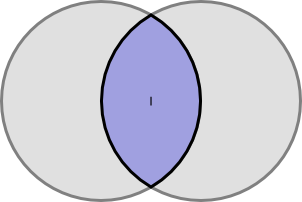
\includegraphics[height=3.03cm]{Figures/1Chapter/intersection}
\end{psfrags}
\caption{The intersection of sets $S$ and $T$ only contains elements that are both in $S$ and $T$.}
\end{center}
\end{figure}

When $S$ and $T$ have no elements in common, we write $S \cap T = \emptyset$.
We also express this fact by saying that $S$ and $T$ are \emph{disjoint}.\index{Disjoint sets}
More generally, a collection of sets is said to be disjoint if no two sets have a common element.
A collection of sets is said to form a \emph{partition} of $S$ if the sets in the collection are disjoint and their union is $S$.\index{Partition}

\begin{figure}[htb]
\begin{center}
\includegraphics[height=3.03cm]{Figures/1Chapter/setpartition}
\caption{A partition of $S$ is a collection of sets that are disjoint and whose union is $S$.}
\end{center}
\end{figure}

The \emph{difference} of two sets, denoted by $S - T$, is defined as the set consisting of those elements of $S$ that are not in $T$, $S - T = \{ x | x \in S \text{ and } x \notin T \}$.
This set is sometimes called the complement of $T$ relative to $S$, or the complement of $T$ in $S$.

\begin{figure}[htb]
\begin{center}
\begin{psfrags}
\psfrag{D}[c]{$S - T$}
\includegraphics[height=3.03cm]{Figures/1Chapter/difference}
\end{psfrags}
\caption{The complement of $T$ relative to $S$ contains all the elements of $S$ that are not in $T$.}
\end{center}
\end{figure}

So far, we have looked at the definition of the union and the intersection of two sets.
We can also form the union or the intersection of arbitrarily many sets.
This is defined in a straightforward way,
\begin{align*}
\bigcup_{\alpha \in \IndexSet} S_{\alpha}
&= \{ x | x \in S_{\alpha} \text{ for some } \alpha \in \IndexSet \} \\
\bigcap_{\alpha \in \IndexSet} S_{\alpha}
&= \{ x | x \in S_{\alpha} \text{ for all } \alpha \in \IndexSet \} .
\end{align*}
The index set $\IndexSet$ can be finite or infinite.


\section{Additional Rules and Properties}

Given a collection of sets, it is possible to form new ones by applying elementary set operations to them.
As in algebra, one uses parentheses to indicate precedence.
For instance, $R \cup (S \cap T)$ denotes the union of two sets $R$ and $S \cap T$, whereas $(R \cup S) \cap T$ represents the intersection of two sets $R \cup S$ and $T$.
The sets thus formed are quite different.

\begin{figure}[htb]
\begin{center}
\begin{psfrags}
\psfrag{P1}[c]{$R \cup (S \cap T)$}
\psfrag{P2}[c]{$(R \cup S) \cap T$}
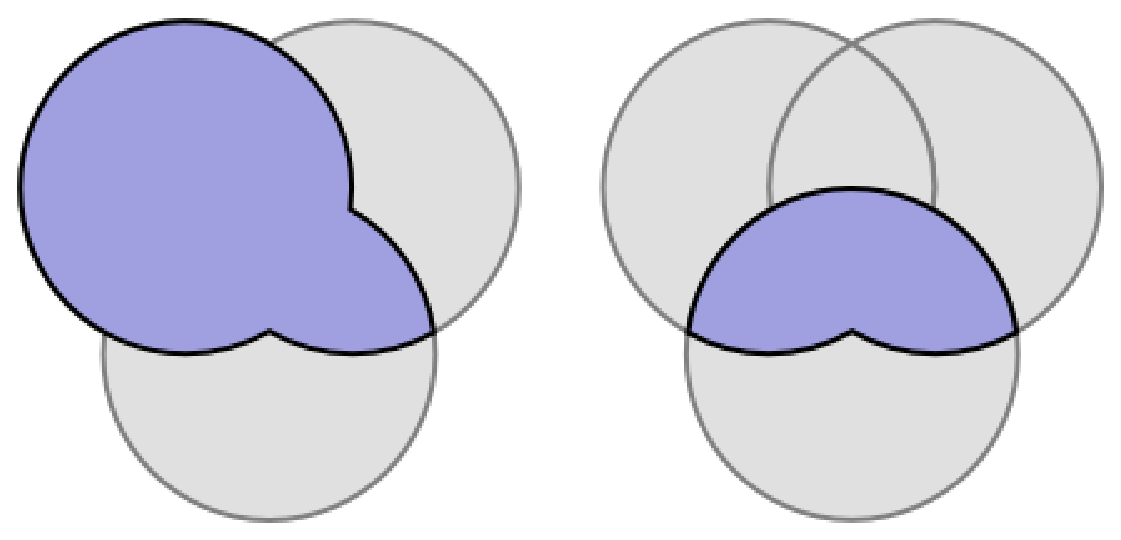
\includegraphics[height=4.55cm]{Figures/1Chapter/triple}
\end{psfrags}
\caption{The order of set operations is important; parentheses should be employed to specify precedence.}
\end{center}
\end{figure}

Sometimes different combinations of operations lead to a same set.
For instance, we have the following distributive laws
\begin{align*}
R \cap (S \cup T) &= (R \cap S) \cup (R \cap T) \\
R \cup (S \cap T) &= (R \cup S) \cap (R \cup T).
\end{align*}
Two particularly useful equivalent combinations of operations are given by \emph{De~Morgan's laws}, which state that\index{De Morgan's laws}
\begin{align*}
R - (S \cup T) &= (R - S) \cap (R - T) \\
R - (S \cap T) &= (R - S) \cup (R - T).
\end{align*}
These two laws can be generalized to
\begin{align*}
\left( \bigcup_{\alpha \in \IndexSet} S_{\alpha} \right)^{\Complement}
&= \bigcap_{\alpha \in \IndexSet} S_{\alpha}^{\Complement} \\
\left( \bigcap_{\alpha \in \IndexSet} S_{\alpha} \right)^{\Complement}
&= \bigcup_{\alpha \in \IndexSet} S_{\alpha}^{\Complement}
\end{align*}
when multiple sets are involved.
To establish the first equality, suppose that $x$ belongs to $\left( \bigcup_{\alpha \in \IndexSet} S_{\alpha} \right)^{\Complement}$.
Then $x$ is not contained in $\bigcup_{\alpha \in \IndexSet} S_{\alpha}$.
That is, $x$ is not an element of $S_{\alpha}$ for any $\alpha \in \IndexSet$.
This implies that $x$ belongs to $S_{\alpha}^{\Complement}$ for all $\alpha \in \IndexSet$, and therefore $x \in \bigcap_{\alpha \in \IndexSet} S_{\alpha}^{\Complement}$.
We have shown that $\left( \bigcup_{\alpha \in \IndexSet} S_{\alpha} \right)^{\Complement} \subset \bigcap_{\alpha \in \IndexSet} S_{\alpha}^{\Complement}$.
The converse inclusion is obtained by reversing the above argument.
The second law can be obtained in a similar fashion.


\section{Cartesian Products}

There is yet another way to create new sets form existing ones.
It involves the notion of an \emph{ordered pair} of objects.\index{Ordered pair}
Given sets $S$ and $T$, the \emph{cartesian product} $S \times T$ is the set of all ordered pairs $(x, y)$ for which $x$ is an element of $S$ and $y$ is an element of $T$, $S \times T = \{ (x, y) | x \in S \text{ and } y \in T \}$.\index{Cartesian product}

\begin{figure}[htb]
\begin{center}
\begin{psfrags}
\psfrag{1}[c]{$1$}
\psfrag{2}[c]{$2$}
\psfrag{3}[c]{$3$}
\psfrag{a}[c]{$a$}
\psfrag{b}[c]{$b$}
\includegraphics[height=3.06cm]{Figures/1Chapter/cartesianproduct}
\end{psfrags}
\caption{Cartesian products can be used to create new sets.
In this example, the sets $\{ 1, 2, 3 \}$ and $\{ a, b \}$ are employed to create a cartesian product with six elements.}
\end{center}
\end{figure}


\section{Set Theory and Probability}

Set theory provides a rigorous foundation for modern probability and its axiomatic basis.
It is employed to describe the laws of probability, give meaning to their implications and answer practical questions.
Being familiar with basic definitions and set operations is key in understanding the subtleties of probability; it helps overcome its many challenges.
A working knowledge of set theory becomes critical when modeling measured quantities and evolving processes that appear random, an invaluable skill for engineers.


\chapter{Concepts of Probability Theory}

The theory of probability provides the mathematical tools necessary to study and analyze uncertain phenomena that occur in nature.
It establishes a formal framework to understand and predict the outcome of a random experiment.
It can also be used to model complex systems and characterize stochastic processes.
This is instrumental in designing efficient solutions to many engineering problems.
Two components define a probabilistic model, a sample space and a probability law.


\section{Sample Spaces and Events}

In the context of probability theory, an \emph{experiment} is a random process that produces one of several \emph{outcomes}. \index{Experiment} \index{Outcome}
The set of all possible outcomes is called the \emph{sample space} of the experiment, and it is denoted by $\Omega$. \index{Sample space}
An \emph{admissible} subset of the sample space is called an \emph{event}. \index{Event}

\begin{center}  % More work needed with figure.
\begin{psfrags}
\psfrag{1}[c]{$1$}
\psfrag{2}[c]{$2$}
\psfrag{3}[c]{$3$}
\psfrag{4}[c]{$4$}
\psfrag{5}[c]{$5$}
\psfrag{6}[c]{$6$}
\psfrag{7}[c]{$7$}
\psfrag{S}[l]{Sample Space $\Omega$}
\psfrag{E}[l]{One Event}
\psfrag{O}[r]{One Outcome}
\includegraphics[height=4.85cm]{Figures/2Chapter/samplespace}
\end{psfrags}
\end{center}

\begin{example}
The rolling of a die forms a common experiment.
The sample space $\Omega$ corresponding to this experiment is given by the six faces of a die.
The set of prime numbers less than or equal to six, namely $\{ 2, 3, 5 \}$, is one of many possible events.
The actual number observed after rolling the die is the outcome of the experiment.

\begin{center}
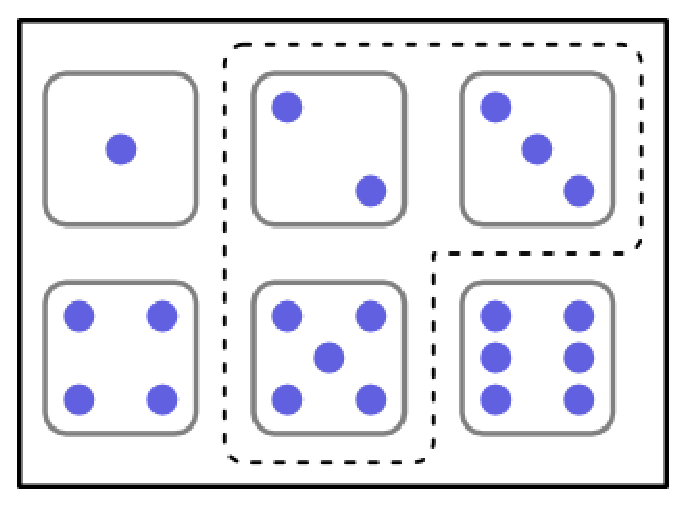
\includegraphics[height=3.375cm]{Figures/2Chapter/dices}
\end{center}
\end{example}

There is essentially no restriction on what constitutes an experiment.
The flipping of a coin, the flipping of $n$ coins, and the flipping of an infinite sequence of coins are all random experiments.
Also, two similar experiments may have different sample spaces.
The sample space $\Omega$ for observing the number of heads in $n$ tosses of a coin is $\{ 0, 1, \ldots, n \}$; whereas for describing the complete history of the $n$ coin tosses, the sample space becomes much larger with $2^n$ distinct sequences of heads and tales.
Ultimately, the choice of a particular sample space depends on the properties one wishes to observe.
Yet some rules must be followed in selecting a sample space.
\begin{enumerate}
\item The elements of a sample space should be \emph{distinct} and \emph{mutually exclusive}. \index{Distinct} \index{Mutually exclusive}
This insures that the outcome of an experiment is unique.
\item A sample space must be \emph{collectively exhaustive}. \index{Collectively exhaustive}
That is, every possible outcome of the experiment must be accounted for in the sample space.
\end{enumerate}
The sample space should be detailed enough to distinguish between all outcomes of interest, while avoiding frivolous details.

\begin{example}
Consider the space composed of the odd integers contained between one and six, the even integers contained between one and six, and the prime numbers less than or equal to six.
This space cannot be a sample space for the rolling of a die since its elements are not mutually exclusive.
In particular, the numbers three and five are both odd and prime, while the number two is prime and even.
This violates the uniqueness criterion.

\begin{center}
\includegraphics[height=4.125cm]{Figures/2Chapter/nonadmissiblespace}
\end{center}

Alternatively, the elements of the space composed of the odd numbers between one and six, and the even numbers between one and six, are distinct and mutually exclusive;
an integer cannot be simultaneously even and odd.
Furthermore, this space is collectively exhaustive since every integer between one and six is either even or odd.
This latter space is a possible sample space for the rolling of a die.

\begin{center}
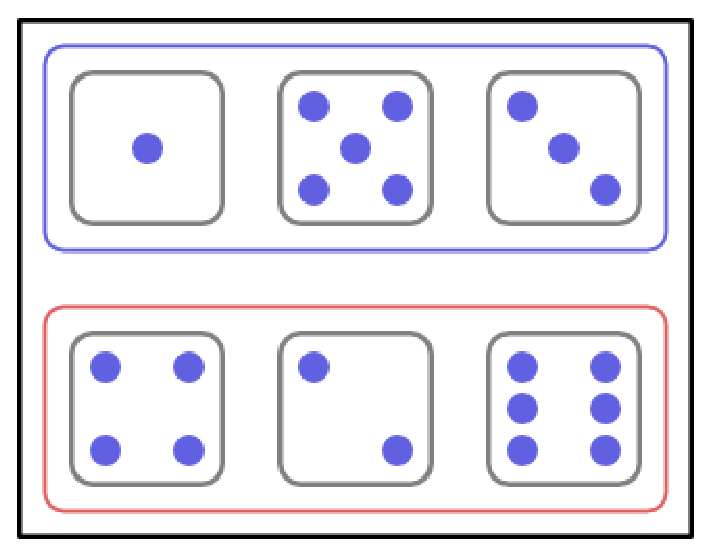
\includegraphics[height=3.75cm]{Figures/2Chapter/admissiblespace}
\end{center}
\end{example}


\section{Probability Laws}
\label{section:ProbabilityLaws}

A \emph{probability law} specifies the likelihood of any event related to an experiment. \index{Probability law}
Formally, a probability law assigns to every event $A$ a number $\Pr (A)$, called the \emph{probability of event $A$}, such that the following axioms are satisfied.
\begin{enumerate}
\item \textbf{(Nonnegativity)} $\Pr (A) \geq 0$, for every event $A$.
\item \textbf{(Normalization)} The probability of the sample space $\Omega$ is equal to one,
\begin{equation*}
\Pr (\Omega) = 1 .
\end{equation*}
\item \textbf{(Countable Additivity)} If $A$ and $B$ are disjoint events with $A \cap B = \emptyset$, then the probability of their union satisfies
\begin{equation*}
\Pr (A \cup B) = \Pr (A) + \Pr(B) .
\end{equation*}
More generally, if $A_1, A_2, \ldots$ is a sequence of disjoint events and $\bigcup_{k=1}^{\infty} A_k$ is itself an admissible event then
\begin{equation*}
\Pr \left( \bigcup_{k=1}^{\infty} A_k \right)
= \sum_{k = 1}^{\infty} \Pr (A_k) .
\end{equation*}
\end{enumerate}

A number of properties can be deduced from the three axioms of probability.
We prove two such properties below.
The first property describes the relation between inclusion and probabilities.
\begin{proposition}
If $A \subset B$, then $\Pr (A) \leq \Pr (B)$.
\end{proposition}
Since $A \subset B$, we have $B = A \cup (B - A)$.
Noting that $A$ and $B - A$ are disjoint sets, we get
\begin{equation*}
\Pr (B) = \Pr (A) + \Pr (B - A) \geq \Pr (A) ,
\end{equation*}
where the inequality follows from the nonnegativity of probability laws.

\begin{center}
\begin{psfrags}
\psfrag{A}[c]{$A$}
\psfrag{B}[l]{$B$}
\psfrag{D}[l]{$B - A$}
\includegraphics[height=3.03cm]{Figures/2Chapter/subset}
\end{psfrags}
\end{center}

The second property specifies the probability of the union of two events that are not necessarily mutually exclusive.
\begin{proposition}
$\Pr (A \cup B) = \Pr (A) + \Pr (B) - \Pr (A \cap B)$.
\end{proposition}

Using the third axiom of probability on the disjoint sets $A$ and $(A \cup B) - A$, we can write
\begin{equation*}
\Pr (A \cup B)
= \Pr (A) + \Pr ((A \cup B) - A)
= \Pr (A) + \Pr (B - A) .
\end{equation*}
Similarly, applying the third axiom to $A \cap B$ and $B - (A \cap B)$, we obtain
\begin{equation*}
\Pr (B)
= \Pr (A \cap B) + \Pr (B - (A \cap B))
= \Pr (A \cap B) + \Pr (B - A) .
\end{equation*}
Combining these two equations yields the desired result.

\begin{center}
\begin{psfrags}
\psfrag{A}[r]{$A$}
\psfrag{B}[l]{$B$}
\psfrag{I}[c]{$A \cap B$}
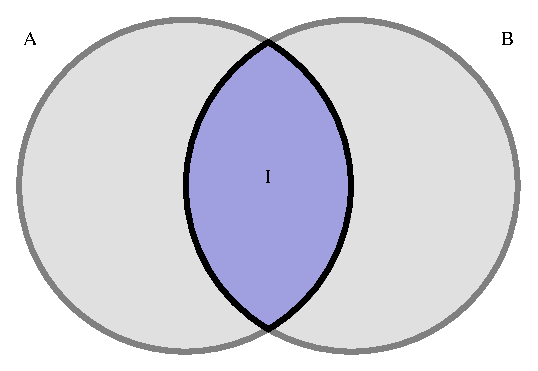
\includegraphics[height=3.03cm]{Figures/2Chapter/intersection}
\end{psfrags}
\end{center}


\subsection{Finite Sample Spaces}

If a sample space $\Omega$ contains a finite number of elements, then a probability law on $\Omega$ is determined completely by the probabilities of individual outcomes.
Denote a sample space $\Omega$ containing $n$ elements by $\Omega = \{ s_1, s_2, \ldots, s_n \}$.
Any event in $\Omega$ is of the form $A = \{ s_i \in \Omega | i \in \IndexSet \}$, where $\IndexSet$ is a subset of the integers one through $n$.
The probability of event $A$ is therefore given by the third axiom of probability,
\begin{equation*}
\Pr (A)
= \Pr ( \{ s_i \in \Omega | i \in \IndexSet \} )
= \sum_{i \in \IndexSet} \Pr (s_i) .
\end{equation*}
Note that, by definition, distinct outcomes are always disjoint events.

If in addition all the elements of $\Omega$ are equally likely with
\begin{equation*}
\Pr (s_1) = \Pr (s_2) = \cdots = \Pr (s_n) = \frac{1}{n} ,
\end{equation*}
then the probability of an event $A$ becomes
\begin{equation*}
\Pr (A) = \frac{ |A| }{n}
= \frac{ \text{number of elements in $A$} }{n} .
\end{equation*}

\begin{example}
The rolling of a fair die is an experiment with a finite number of equally likely outcomes.
The probability of observing any of the faces labeled one through six is $1/6$.
The probability of any event can easily be computed by counting the number of distinct outcomes included in the event.
For instance, the probability of rolling a prime number is
\begin{equation*}
\Pr (\text{outcome is prime})
= \Pr ( \{ 2, 3, 5 \} )
= \Pr (2) + \Pr(3) + \Pr(5) = \frac{3}{6} .
\end{equation*}
\end{example}


\subsection{Countably Infinite Models}

Consider a sample space that consists of a countably infinite number of elements, $\Omega = \{ s_1, s_2, \ldots \}$.
Again, a probability law on $\Omega$ is specified by the probabilities of individual outcomes.
An event in $\Omega$ can be written as $A = \{ s_j \in \Omega | j \in \JndexSet \}$, where $\JndexSet$ is a subset of the positive integers.
Using the third axiom of probability, $\Pr (A)$ is given by
\begin{equation*}
\Pr (A)
= \Pr ( \{ s_j \in \Omega | j \in \JndexSet \} )
= \sum_{j \in \JndexSet} \Pr (s_j) .
\end{equation*}
The possibly infinite sum $\sum_{j \in \JndexSet} \Pr (s_j)$ always converges since the summands are nonnegative and the sum is bounded above by one.
It is therefore well-defined.

\begin{example} \label{example:CoinTossSequence}
Suppose that a fair coin is tossed repetitively until heads is observed.
The number of coin tosses is recorded as the outcome of this experiment.
The sample space for this experiment is $\Omega = \{ 1, 2, \ldots \}$, a countably infinite set.

\begin{center}
\begin{psfrags}
\psfrag{1}[c]{$1$}
\psfrag{2}[c]{$2$}
\psfrag{3}[c]{$3$}
\psfrag{4}[c]{$4$}
\psfrag{5}[c]{$5$}
\psfrag{6}[c]{$6$}
\psfrag{7}[c]{$7$}

\includegraphics[height=0.765cm]{Figures/2Chapter/countablespace}
\end{psfrags}
\end{center}

The probability of observing heads on the first trial is $0.5$, and the probability of observing heads for the first time on trial $k$ is $2^{-k}$.
The probability of the entire sample space is equal to
\begin{equation*}
\Pr ( \Omega ) = \sum_{k=1}^{\infty} \Pr (k)
= \sum_{k=1}^{\infty} \frac{1}{2^k} = 1 ,
\end{equation*}
as expected.
Similarly, the probability of the number of coin tosses being even can be computed as
\begin{equation*}
\Pr ( \text{outcome is even} )
= \sum_{k=1}^{\infty} \Pr (2k)
= \sum_{k = 1}^{\infty} \frac{1}{2^{2k}}
= \frac{1}{4} \frac{1}{ \left( 1 - \frac{1}{4} \right) }
= \frac{1}{3} .
\end{equation*}
\end{example}


\subsection{Uncountably Infinite Models}

Probabilistic models with uncountably infinite sample spaces differ from the finite and countable cases in that a probability law may not necessarily be specified by the probability of single-element outcomes.
This difficulty arises from the large number of elements contained in the sample space $\Omega$ when the latter is uncountable.
Many subsets of $\Omega$ do not have a finite or countable representation, and as such the third axiom of probability cannot be applied to relate the probabilities of these events to the probabilities of individual outcomes.
Despite these apparent difficulties, probabilistic models with uncountably infinite sample spaces are extremely useful in practice.
To develop an understanding of uncountable probabilistic models, we consider the unit interval $[0, 1]$.

\begin{center}
\begin{psfrags}
\psfrag{0}[c]{$0$}
\psfrag{1}[c]{$1$}
\includegraphics[height=1.17cm]{Figures/2Chapter/uncountablespace}
\end{psfrags}
\end{center}

Suppose that one element is chosen at random from this interval, and that all the elements are equally likely.
By the first axiom of probability, we have $\Pr \left( [0,1] \right) = 1$.
Furthermore, if two intervals have the same length, the probabilities of the outcome falling in either interval should be identical.
For instance,
$\Pr \left( \left( 0, 0.25 \right) \right)
= \Pr \left( \left( 0.75, 1 \right) \right)$.

\begin{center}
\begin{psfrags}
\psfrag{0}[l]{$0$}
\psfrag{0.25}[r]{$0.25$}
\psfrag{0.75}[l]{$0.75$}
\psfrag{1}[r]{$1$}
\includegraphics[height=1.18cm]{Figures/2Chapter/intervals}
\end{psfrags}
\end{center}

In an extension of the previous observation, we define the probability of an open interval $(a, b)$ where $0 \leq a < b \leq 1$ by
\begin{equation} \label{equation:DefinitionProbabilityLaw1}
\Pr ( (a,b) ) = b - a .
\end{equation}
Using the third axiom of probability, it is then possible to find the probability of a finite or countable union of disjoint open intervals.

\begin{center}
\begin{psfrags}
\psfrag{0}[l]{$0$}
\psfrag{1}[r]{$1$}
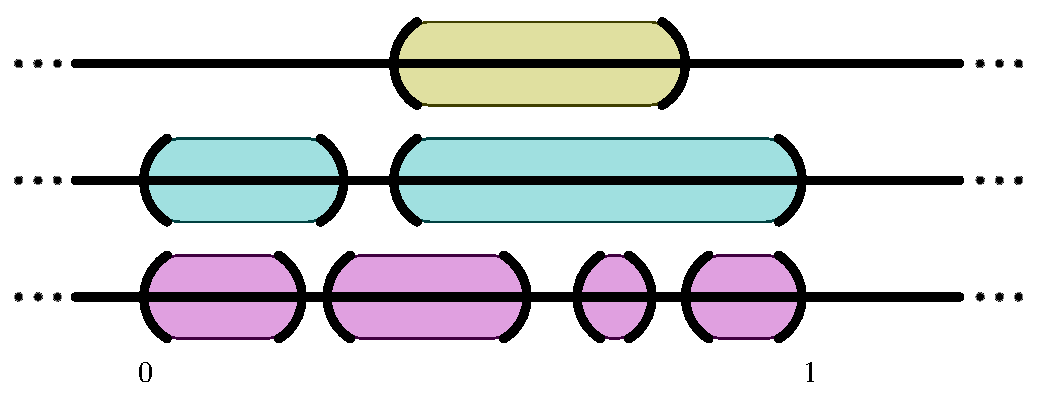
\includegraphics[height=3.285cm]{Figures/2Chapter/lineintervals}
\end{psfrags}
\end{center}

Specifically, for constants $0 \leq a_1 < b_1 < a_2 < b_2 < \cdots \leq 1$, we get
\begin{equation*}
\Pr \left( \bigcup_{k=1}^{\infty} (a_k,b_k) \right)
= \sum_{k=1}^{\infty} b_k - a_k .
\end{equation*}
The probabilities of more complex events can be obtained by considering additional elementary set operations.
However, it suffices to say for now that specifying the probability of the outcome falling in $(a,b)$ for every possible open interval is enough to define a probability law on $\Omega$.
In the example at hand, \eqref{equation:DefinitionProbabilityLaw1} completely determines the probability law on $[0,1]$.

Note that we can give an alternative means of computing the probability of an interval.
Again, consider the open interval $(a, b)$ where $0 \leq a < b \leq 1$.
The probability of the outcome falling in this  interval is equal to
\begin{equation*}
\Pr ( (a, b) ) = b - a = \int_a^b dx = \int_{(a,b)} dx .
\end{equation*}
Moreover, for $0 \leq a_1 < b_1 < a_2 < b_2 < \cdots \leq 1$, we can write
\begin{equation*}
\Pr \left( \bigcup_{k=1}^{\infty} (a_k,b_k) \right)
= \sum_{k=1}^{\infty} \left( b_k - a_k \right)
= \int_{\bigcup_{k=1}^{\infty} (a_k,b_k)} dx .
\end{equation*}
For this carefully crafted example, it appears that the probability of an admissible event $A$ is given by the integral
\begin{equation*}
\Pr (A) = \int_{A} dx .
\end{equation*}
This is indeed accurate for the experiment at hand.
In fact, the class of admissible events for this experiment is simply the collection of all sets for which the integral $\int_A dx$ can be computed.
In other words, if a number is chosen at random from $[0,1]$, then the probability of this number falling in the measurable set $A \subset [0,1]$ is
\begin{equation*}
\Pr (A) = \int_{A} dx .
\end{equation*}
In this document, we will see many probabilistic models with uncountably infinite sample spaces.
The mathematical tools required to handle such models will be treated alongside.

\begin{example}
Suppose that a participant at a game-show is required to spin the wheel of misfortune, a perfect circle with unit circumference.
When subjected to a vigorous spin, the wheel is equally likely to stop anywhere along its periphery.
The sampling space for this experiment is $[0, 1)$, an uncountable set.
Its probability is given by $\Pr ([0, 1)) = 1$.

\begin{center}
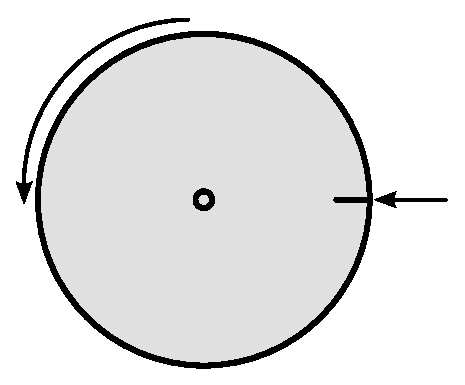
\includegraphics[height=3.15cm]{Figures/2Chapter/wheel}
\end{center}

The probability that the wheel stops in the first quadrant is given by
\begin{equation*}
\Pr \left( \left[ 0, \frac{1}{4} \right) \right) = \frac{1}{4}.
\end{equation*}
Similarly, the probability that the wheel stops in an interval $(a, b)$ where $0 \leq a \leq b < 1$ is
\begin{equation*}
\Pr ((a,b)) = b - a.
\end{equation*}
If $B \subset [0, 1)$ is the measurable set representing a winning outcome, then the probability of success at the wheel is
\begin{equation*}
\Pr(B) = \int_B dy .
\end{equation*}
\end{example}


\subsection{Probability and Measure Theory*}

A systematic treatment of probability involves advanced mathematical concepts.
The basis of our intuition for the infinite is the set of natural numbers,
\begin{equation*}
\NaturalNumbers = \{ 1, 2, \ldots \}.
\end{equation*}
Two sets are said to have the same \emph{cardinality} if their elements can be put in one-to-one correspondence. \index{Cardinality}
A set with the same cardinality as the natural numbers is said to be \emph{countable}. \index{Countable}
That is, the elements of a countable set can always be listed in sequence
\begin{equation*}
s_1, s_2, \ldots
\end{equation*}
although the order may have nothing to do with any relation between the elements.
The integers and the rational numbers are examples of countably infinite sets.
It may be surprising at first to learn that there exist uncountable sets.
To escape beyond the countable, one needs set theoretic tools such as \emph{power sets}.
The set of real numbers is uncountably infinite; it cannot be put in one-to-one correspondence with the natural numbers.
A typical progression in analysis consists of using the finite to get at the countably infinite, and then to use the countably infinite to get at the uncountable.

It is tempting to try to assign probabilities to every subset of a sample space $\Omega$.
However, for uncountably infinite sample spaces, this leads to serious difficulties that cannot be resolved.
In general, it is necessary to work with special subclasses of the class of all subsets of a sample space $\Omega$.
The collections of the appropriate kinds are called fields and $\sigma$-fields, and they are defined and studied in \emph{measure theory}. \index{Measure theory}
This leads to measure-theoretic probability, and to its unified treatment of the discrete and the continuous.
Fortunately, it is possible to develop an intuitive and working understanding of probability without worrying about these issues.
At some point of your academic career, you may wish to study analysis and measure theory more carefully and in greater details.
However, it is not our current purpose to initiate the study of these fields.


\chapter{Conditional Probability}
\label{chapter:ConditionalProbability}

Conditional probability provides a way to compute the likelihood of an event based on \emph{partial information}.
This is a powerful concept that is used extensively throughout engineering with applications to decision making, networks and digital communications.


\section{Conditioning on Events}

We begin our discussion of conditional probability with an illustrative example.
The intuition gained through this simple exercise is then generalized by introducing a formal definition for this important concept.

\begin{example}
The rolling of a fair die is an experiment with six equally likely outcomes.
As such, the probability of obtaining any of the outcomes is $1/6$.
However, if we are told that the upper face displays an odd number, then only three possibilities remain, namely $\{1, 3, 5 \}$.

\begin{center}
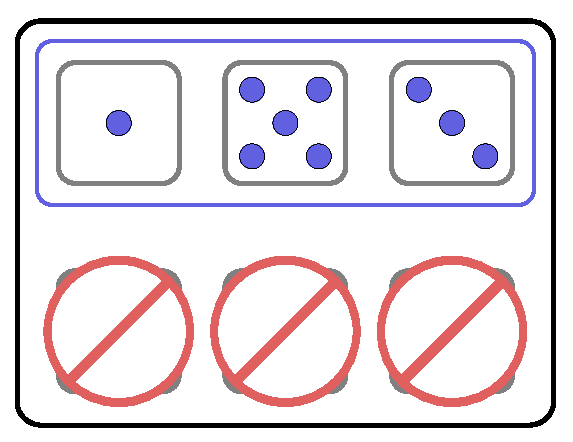
\includegraphics[height=3.675cm]{Figures/3Chapter/condevent}
\end{center}

These three outcomes had equal probabilities before the additional information was revealed.
It is natural to assume that they remain equally likely afterwards.
In particular, it is reasonable to assign a probability of $1/3$ to each of the three outcomes still plausible, in view of the new information.
Note that we can express the probability of getting, say, a three given that the outcome is an odd number as
\begin{equation*}
\begin{split}
\Pr (\text{3 given } \{ \text{odd numbers} \})
&= \frac{\Pr (\text{3 and } \{ \text{odd numbers} \})}
{\Pr (\text{odd numbers})} \\
&= \frac{\Pr(3)}{\Pr (\{1,3,5\})} = \frac{1}{3} .
\end{split}
\end{equation*}
\end{example}

Having reviewed a specific situation, we now turn to the more encompassing setting.
Let $B$ be an event such that $\Pr (B) > 0$.
A conditional probability law assigns to every event $A$ a number $\Pr (A|B)$, termed the \emph{conditional probability of $A$ given $B$}, such that \index{Conditional Probability}
\begin{equation} \label{equation:ConditionalProbability}
\Pr (A | B) = \frac{\Pr (A \cap B)}{\Pr (B)}.
\end{equation}
We can show that the set of conditional probabilities $\{ \Pr (A | B) \}$ specifies a valid probability law, as defined in Section~\ref{section:ProbabilityLaws}.
For every event $A$, we have
\begin{equation*}
\Pr (A|B) = \frac{\Pr (A \cap B)}{\Pr (B)} \geq 0.
\end{equation*}
That is, $\Pr (A|B)$ is nonnegative.
The probability of the entire sample space $\Omega$ is equal to
\begin{equation*}
\Pr (\Omega | B) = \frac{\Pr (\Omega \cap B)}{\Pr (B)}
= \frac{\Pr (B)}{\Pr (B)} = 1 .
\end{equation*}
If $A_1, A_2, \ldots$ is a sequence of disjoint events, then
\begin{equation*}
A_1 \cap B, A_2 \cap B, \ldots
\end{equation*}
is also a sequence of disjoint events and
\begin{equation*}
\begin{split}
\Pr \left( \bigcup_{k=1}^{\infty} A_k \Big| B \right)
&= \frac{\Pr \left( \left( \bigcup_{k=1}^{\infty} A_k \right) \cap B \right)}{\Pr (B)}
= \frac{\Pr \left( \bigcup_{k=1}^{\infty} (A_k \cap B ) \right)}{\Pr (B)} \\
&= \sum_{k = 1}^{\infty} \frac{ \Pr (A_k \cap B ) }{\Pr (B)}
= \sum_{k = 1}^{\infty} \Pr (A_k | B) ,
\end{split}
\end{equation*}
where the third equality follows from the third axiom of probability applied to the set $\bigcup_{k=1}^{\infty} (A_k \cap B )$.
Hence, the conditional probability law defined by \eqref{equation:ConditionalProbability} satisfies the three axioms of probability.

\begin{example}
A fair coin is tossed repetitively until heads is observed.
In Example~\ref{example:CoinTossSequence}, we found that the probability of observing heads for the first time on trial $n$ is $2^{-k}$.
We now wish to compute the probability that heads occurred for the first time on the second trial given that it took an even number of tosses to observe heads.
In this example, $A = \{ 2 \}$ and $B$ is the set of even numbers.
The probability that the outcome is two given that the number of tosses is even is equal to
\begin{equation*}
\begin{split}
\Pr ( 2 | \text{even numbers} )
&= \frac{\Pr ( 2 \cap \{ \text{even numbers} \} )}
{\Pr (\text{even numbers})} \\
&= \frac{\Pr (2)}{\Pr (\text{even numbers})} \\
&= \frac{1/4}{1/3}
= \frac{3}{4} .
\end{split}
\end{equation*}
In the above computation, we have used the fact that the probability of flipping the coin an even number of times is equal to $1/3$.
This fact was obtained in Example~\ref{example:CoinTossSequence}.
\end{example}

The definition of conditional probability can be employed to compute the probability of several events occurring simultaneously.
Let $A_1, A_2, \ldots, A_n$ be a collection of events.
The probability of events $A_1$ through $A_n$ taking place at the same time is given by
\begin{equation} \label{equation:SimultaneousEvents}
\Pr \left( \bigcap_{k=1}^n A_k \right)
= \Pr (A_1) \Pr (A_2 | A_1) \Pr (A_3 | A_1 \cap A_2)
\cdots \Pr \left( A_n \bigg| \bigcap_{k=1}^{n-1} A_k \right) .
\end{equation}
This formula can be verified by expanding each of the conditional probabilities using \eqref{equation:ConditionalProbability},
\begin{equation*}
\Pr \left( \bigcap_{k=1}^n A_k \right)
= \Pr (A_1) \frac{\Pr (A_2 \cap A_1)}{\Pr (A_1)}
\frac{\Pr (A_1 \cap A_2 \cap A_3)}{\Pr (A_1 \cap A_2)}
\cdots \frac{\Pr \left( \bigcap_{k=1}^{n} A_k \right)}
{\Pr \left( \bigcap_{k=1}^{n-1} A_k \right)} .
\end{equation*}

\begin{example}
An urn contains eight blue balls and four green balls.
Three balls are drawn from this urn without replacement.
We wish to compute the probability that all three balls are blue.
The probability of drawing a blue ball the first time is equal to $8/12$.
The probability of drawing a blue ball the second time given that the first ball is blue is $7/11$.
Finally, the probability of drawing a blue ball the third time given that the previous two balls are blue is $6/10$.
Using \eqref{equation:SimultaneousEvents}, we can compute the probability drawing three blue balls as
\begin{equation*}
\Pr (\text{3 blue balls})
= \frac{8}{12} \frac{7}{11} \frac{6}{10}
= \frac{14}{55} .
\end{equation*}

\begin{center}
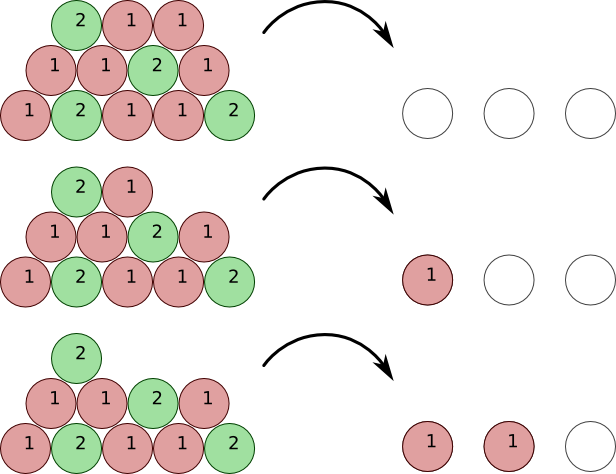
\includegraphics[height=7.11cm]{Figures/3Chapter/balls}
\end{center}
\end{example}


\section{The Total Probability Theorem}

The probability of events $A$ and $B$ occurring at the same time can be calculated as a special case of \eqref{equation:SimultaneousEvents}.
For two events, this computational formula simplifies to
\begin{equation} \label{equation:ProbabilityIntersection}
\Pr (A \cap B) = \Pr (A|B) \Pr (B) .
\end{equation}
We can also obtain this equation directly from the definition of conditional probability.
This property is a key observation that plays a central role in establishing two important results, the \emph{total probability theorem} and \emph{Bayes' rule}.
To formulate these two theorems, we need to revisit the notion of a partition.
A collection of events $A_1, A_2, \ldots, A_n$ is said to be a \emph{partition} of the sample space $\Omega$ if these events are disjoint and their union is the entire sample space, \index{Partition}
\begin{equation*}
\bigcup_{k=1}^n A_k = \Omega .
\end{equation*}
Visually, a partition divides an entire set into disjoint subsets.
\begin{center}
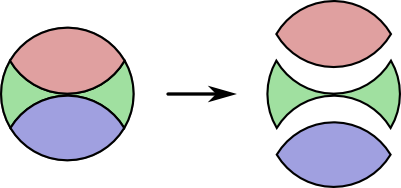
\includegraphics[height=4.23cm]{Figures/3Chapter/setpartition2}
\end{center}

\begin{theorem}[Total Probability Theorem] \label{theorem:TotalProbability} \index{Total Probability Theorem}
Let $A_1, A_2, \ldots, A_n$ be a collection of events that forms a partition of the sample space $\Omega$.
Suppose that $\Pr (A_k) > 0$ for all $k$.
Then, for any event $B$, we can write
\begin{equation*}
\begin{split}
\Pr (B) &= \Pr (A_1 \cap B) + \Pr (A_2 \cap B) + \cdots + \Pr (A_n \cap B) \\
&= \Pr (A_1) \Pr (B | A_1) + \Pr (A_2) \Pr (B | A_2) + \cdots + \Pr (A_n) \Pr (B | A_n ) .
\end{split}
\end{equation*}
\end{theorem}
\begin{proof}
The collection of events $A_1, A_2, \ldots, A_n$ forms a partition of the sample space $\Omega$.
We can therefore write
\begin{equation*}
B = B \cap \Omega = B \cap \left( \bigcup_{k=1}^n A_k \right) .
\end{equation*}
Since $A_1, A_2, \ldots, A_n$ are disjoint sets, the events
\begin{equation*}
A_1 \cap B, A_2 \cap B, \ldots, A_n \cap B
\end{equation*}
are also disjoint.
Combining these two facts, we get
\begin{equation*}
\begin{split}
\Pr (B)
&= \Pr \left( B \cap \left( \bigcup_{k=1}^n A_k \right) \right)
= \Pr \left( \bigcup_{k=1}^n (B \cap A_k) \right) \\
&= \sum_{k=1}^n \Pr \left( B \cap A_k \right)
= \sum_{k=1}^n \Pr (A_k) \Pr \left( B |A_k \right) ,
\end{split}
\end{equation*}
where the fourth equality is obtained by applying the third axiom of probability.
\end{proof}

\begin{center}
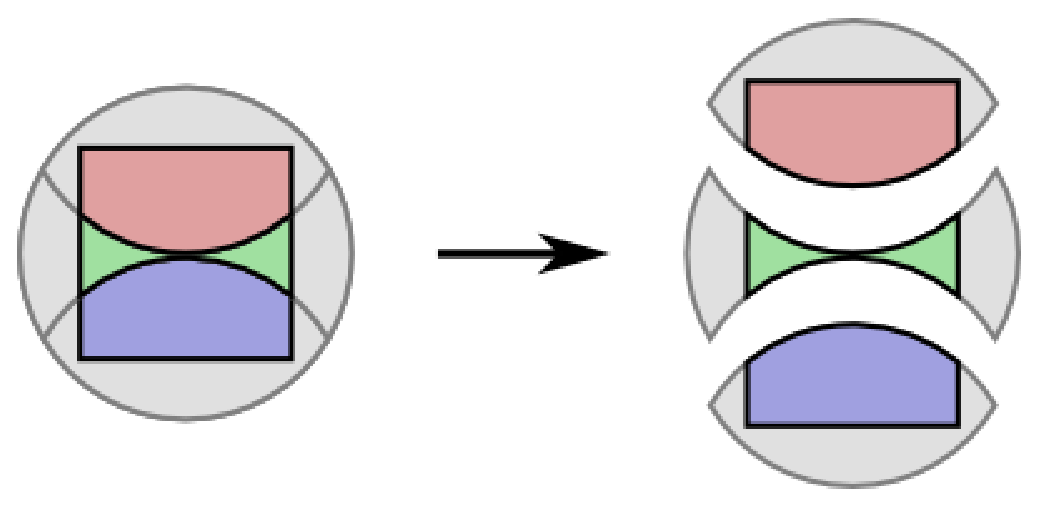
\includegraphics[height=4.23cm]{Figures/3Chapter/setpartition3}
\end{center}
A graphical interpretation of Theorem~\ref{theorem:TotalProbability} is illustrated above.
Event $B$ can be decomposed into the disjoint union of $A_1 \cap B, A_2 \cap B, \ldots, A_n \cap B$.
The probability of event $B$ can then be computed by adding these various parts
\begin{equation*}
\Pr (A_1 \cap B), \Pr (A_2 \cap B), \ldots, \Pr (A_n \cap B) .
\end{equation*}

\begin{example}
An urn contains eight blue balls and four red balls.
A first ball is drawn from the urn.
If this ball is red then the experiment stops, otherwise one more ball is drawn from the urn.
What is the probability of obtaining a red ball?

In this problem, there are three outcomes of interest.
If we denote the drawing of a red ball by $r$ and the drawing of a blue ball by $b$, then these three outcomes can be represented by $\{ r, br, bb \}$.
The probability of drawing a red ball initially is $\Pr (r) = 4/12$.
The probabilities of drawing two balls can be computed using \eqref{equation:SimultaneousEvents}, and they are given by
\begin{align*}
\Pr (br) &= \frac{8}{12} \frac{4}{11} = \frac{8}{33} \\
\Pr (bb) &= \frac{8}{12} \frac{7}{11} = \frac{14}{33} .
\end{align*}
Let $R$ denote the event that a red ball is obtained during the experiment.
The overall probability of getting a red ball, $\Pr (R)$, can be computed by applying the total probability theorem
\begin{equation*}
\begin{split}
\Pr (R) &= \Pr (R \cap r) + \Pr (R \cap br) + \Pr (R \cap bb) \\
&= \Pr(r) \Pr (R|r) + \Pr(br) \Pr (R|br) + \Pr(bb) \Pr (R|bb) \\
&= \frac{1}{3} \cdot 1 + \frac{8}{33} \cdot 1 + \frac{14}{33} \cdot 0
= \frac{19}{33} .
\end{split}
\end{equation*}
\end{example}


\section{Bayes' Rule}

The following result is also very useful.
It relates the conditional probability of $A$ given $B$ to the conditional probability of $B$ given $A$.

\begin{theorem}[Bayes' Rule] \index{Bayes' Rule}
Let $A_1, A_2, \ldots, A_n$ be a collection of events that forms a partition of the sample space $\Omega$.
Suppose that $\Pr (A_k) > 0$ for all $k$.
Then, for any event $B$ such that $\Pr (B) > 0$, we can write
\begin{equation*}
\begin{split}
\Pr (A_i | B)
&= \frac{ \Pr (A_i) \Pr (B | A_i) }{ \Pr (B) } \\
&= \frac{ \Pr (A_i) \Pr (B | A_i) }
{ \sum_{k=1}^n \Pr (A_k) \Pr (B | A_k) } .
\end{split}
\end{equation*}
\end{theorem}
\begin{proof}
Bayes' rule is easily verified.
We expand the probability of $A_i \cap B$ using \eqref{equation:ProbabilityIntersection} twice, and we get
\begin{equation*}
\Pr (A_i \cap B) = \Pr (A_i | B) \Pr (B) = \Pr (B | A_i) \Pr (A_i).
\end{equation*}
Rearranging the terms yields the first equality.
The second equality is obtained by writing
\begin{equation*}
\begin{split}
\Pr (B) &= \Pr (B \cap \Omega)
= \Pr \left( B \cap \left( \bigcup_{k=1}^n A_k \right) \right) \\
&= \sum_{k=1}^n \Pr (B \cap A_k)
= \sum_{k=1}^n \Pr (A_k) \Pr (B | A_k) .
\end{split}
\end{equation*}
The application of the third axiom of probability is justified because
\begin{equation*}
A_1, A_2, \ldots, A_n
\end{equation*}
are disjoint events.
\end{proof}

\begin{example}
April, a biochemist, designs a test for a latent disease.
If a subject has the disease, the probability that the test results are positive is $0.95$.
Similarly, if a subject does not have the disease, the probability that the test results are negative is $0.95$.
Suppose that one percent of the population has the disease.
We wish to find the probability that a person who tested positive has the disease.

Let $D$ denote the event that the person has the disease, and let $P$ be the event that the test results are positive.
Using Bayes' rule, we can easily compute the probability that a person who tested positive has the disease,
\begin{equation*}
\begin{split}
\Pr (D|P)
&= \frac{ \Pr(D) \Pr(P|D) }{ \Pr(D) \Pr(P|D) + \Pr(D^{\Complement}) \Pr(P|D^{\Complement}) } \\
&= \frac{ 0.01 \cdot 0.95 }{ 0.01 \cdot 0.95 + 0.99 \cdot 0.05 } \\
&\approx 0.1610 .
\end{split}
\end{equation*}
Although the test is fairly accurate, the probability that a person with a positive test carries the disease remains small.
\end{example}


\section{Independence}
\label{section:Independence}

Events $A$ and $B$ are said to be \emph{independent} if $\Pr (A \cap B) = \Pr(A) \Pr(B)$. \index{Independence}
Interestingly, independence is closely linked to the concept of conditional probability.
If $\Pr(B) > 0$ and events $A$ and $B$ are independent, then
\begin{equation*}
\Pr (A | B) = \frac{ \Pr (A \cap B) }{\Pr (B)}
= \frac{ \Pr (A) \Pr(B) }{\Pr (B)}
= \Pr (A).
\end{equation*}
The \emph{a priori} probability of event $A$ is identical to the \emph{a posteriori} probability of $A$ given $B$.
That is, if $A$ is independent of $B$, then partial knowledge about $B$ contains no information on the likely occurrence of $A$.
We note that independence is a symmetric relation; if $A$ is independent of $B$, then $B$ is also independent of $A$.
It is therefore unambiguous to say that $A$ and $B$ are independent events.

\begin{example}
Suppose that two dice are rolled at the same time, a red die and a blue die.
We observe the numbers that appear on the upper faces of the two dice.
The sample space for this experiment is composed of thirty-six equally likely outcomes.
Consider the probability of getting a four on the red die given that the blue die shows a six,
\begin{equation*}
\begin{split}
\Pr (\text{red = 4} | \text{blue = 6})
&= \frac{ \Pr (\text{red = 4} \cap \text{blue = 6}) }
{ \Pr (\text{blue = 6}) } \\
&= \frac{1}{6} = \Pr (\text{red = 4}) .
\end{split}
\end{equation*}
From this equation, we gather that
\begin{equation*}
\Pr (\text{red = 4} \cap \text{blue = 6})
= \Pr (\text{red = 4}) \Pr (\text{blue = 6}) .
\end{equation*}
Thus, rolling a four on the red die and rolling a six on the blue die are independent events.

Similarly, consider the probability of obtaining a four on the red die given that the sum of the two dice is eleven,
\begin{equation*}
\begin{split}
\Pr (\text{red = 4} | \text{sum = 11})
&= \frac{ \Pr (\text{red = 4} \cap \text{sum = 11}) }
{ \Pr (\text{sum = 11}) } = 0 \\
&\neq \frac{1}{6} = \Pr (\text{red = 4}) .
\end{split}
\end{equation*}
In this case, we conclude that getting a four on the red die and a sum total of eleven are not independent events.
\end{example}

The basic idea of independence seems intuitively clear: if knowledge about the occurrence of event $B$ has no impact on the probability of $A$, then these two events must be independent.
Yet independent events are not necessarily easy to visualize in terms of the sample space.
A common mistake is to assume that two events are independent if they are disjoint.
Two mutually exclusive events can hardly be independent.
If $\Pr (A) > 0$, $\Pr (B) > 0$, and $\Pr (A \cap B) = 0$ then
\begin{equation*}
\Pr (A \cap B) = 0 < \Pr (A) \Pr(B).
\end{equation*}
Thus, $A$ and $B$ cannot be independent if they are disjoint, non-trivial sets.


\subsection{Independence of Multiple Events}

The concept of independence can be extended to multiple events.
The events $A_1, A_2, \ldots, A_n$ are \emph{independent} provided that \index{Independence}
\begin{equation} \label{equation:IndependenceMultipleEvents}
\Pr \left( \bigcap_{i \in \IndexSet} A_i \right)
= \prod_{i \in \IndexSet} \Pr (A_i) ,
\end{equation}
for every subset $\IndexSet$ of $\{1, 2, \ldots, n\}$.

For instance, consider a collection of three events, $A$, $B$ and $C$.
These events are independent if
\begin{equation} \label{equation:ThreeIndependentEvents}
\begin{split}
\Pr (A \cap B) &= \Pr (A) \Pr (B) \\
\Pr (A \cap C) &= \Pr (A) \Pr (C) \\
\Pr (B \cap C) &= \Pr (B) \Pr (C)
\end{split}
\end{equation}
and, in addition,
\begin{equation*}
\Pr (A \cap B \cap C) = \Pr (A) \Pr (B) \Pr(C) .
\end{equation*}
The three equalities in \eqref{equation:ThreeIndependentEvents} assert that $A$, $B$ and $C$ are \emph{pairwise independent}.
Note that the fourth condition does not follow from the first three conditions, nor does it imply any of them.
Pairwise independence does not imply independence.

\begin{example}
A fair coin is flipped twice.
Let $A$ denote the event that heads is observed on the first toss.
Let $B$ be the event that heads is obtained on the second toss.
Finally, let $C$ be the event that the two coins show distinct sides.
These three events each have a probability of $1/2$.
Furthermore, we have
\begin{equation*}
\Pr (A \cap B) = \Pr (A \cap C) = \Pr (B \cap C) = \frac{1}{4} .
\end{equation*}
That is, these events are pairwise independent.
However, we can verify that
\begin{equation*}
\Pr (A \cap B \cap C) = 0 \neq \frac{1}{8} = \Pr (A) \Pr (B) \Pr (C) .
\end{equation*}
This shows that events $A$, $B$ and $C$ are not independent.
\end{example}

\begin{example}
Two dice are rolled at the same time, a red die and a blue die.
Let $A$ be the event that the number on the red die is odd.
Let $B$ be the event that the number on the red die is either two, three or four.
Also, let $C$ be the event that the product of the two dice is twelve.
The individual probabilities of these events are
\begin{align*}
\Pr (A) &= \Pr (\text{red is odd}) = \frac{1}{2} \\
\Pr (B) &= \Pr (\text{red} \in \{2, 3, 4\}) = \frac{1}{2} \\
\Pr (C) &= \Pr (\text{product = 12}) = \frac{4}{36} .
\end{align*}
We note that these events are not pairwise independent because
\begin{align*}
\Pr (A \cap B) &= \frac{1}{6} \neq \frac{1}{4} = \Pr(A) \Pr(B) \\
\Pr (A \cap C) &= \frac{1}{36} \neq \frac{1}{18} = \Pr(A) \Pr(C) \\
\Pr (B \cap C) &= \frac{1}{12} \neq \frac{1}{18} = \Pr(B) \Pr(C) .
\end{align*}
The multiple events $A$, $B$ and $C$ are not independent.
On the other hand, the probability of these three events occurring simultaneously is
\begin{equation*}
\Pr (A \cap B \cap C) = \frac{1}{36}
= \frac{1}{2} \cdot \frac{1}{2} \cdot \frac{4}{36}
= \Pr (A) \Pr (B) \Pr (C) .
\end{equation*}
\end{example}

\subsection{Conditional Independence}

We introduced earlier the meaning of conditional probability, and we showed that the set of conditional probabilities $\{ \Pr (A|B) \}$ specifies a valid probability law.
It is therefore possible to discuss independence with respect to conditional probability.
We say that events $A_1$ and $A_2$ are \emph{conditionally independent} if \index{Conditional Independence}
\begin{equation*}
\Pr (A_1 \cap A_2 | B) = \Pr (A_1 | B) \Pr (A_2 | B) .
\end{equation*}
Note that if $A_1$ and $A_2$ are conditionally independent given event $B$, we can use equation \eqref{equation:ConditionalProbability} to write
\begin{equation*}
\begin{split}
\Pr (A_1 \cap A_2 | B) &= \frac{ \Pr (A_1 \cap A_2 \cap  B) }{\Pr (B)} \\
&= \frac{ \Pr (B) \Pr (A_1 | B) \Pr (A_2 | A_1 \cap  B) }{\Pr (B)} \\
&= \Pr (A_1 | B) \Pr (A_2 | A_1 \cap  B) .
\end{split}
\end{equation*}
Under the assumption that $\Pr (A_1 | B) > 0$, we can combine the previous two expressions and get
\begin{equation*}
\Pr (A_2 | A_1 \cap  B) = \Pr (A_2 | B) .
\end{equation*}
This latter result asserts that, given event $B$ has taken place, the additional information that $A_1$ also occurred does not affect the conditional probability of $A_2$.
It is simple to show that conditional independence is a symmetric relation as well.

\begin{example}
Suppose that a fair coin is tossed until heads is observed.
The number of trials is recorded as the outcome of this experiment.
We denote by $B$ the event that the coin is tossed more than one time.
Moreover, we let $A_1$ be the event that the number of trials is an even number, and $A_2$ be the event that the number of trials is less than six.
The conditional probabilities of $A_1$ and $A_2$ given that the coin is tossed more than once are
\begin{align*}
\Pr (A_1 | B) &= \frac{ \Pr (A_1 \cap B) }{ \Pr (B) }
= \frac{1/3}{1/2} = \frac{2}{3} \\
\Pr (A_2 | B) &= \frac{ \Pr (A_2 \cap B) }{ \Pr (B) }
= \frac{15/32}{1/2} = \frac{15}{16} .
\end{align*}
The joint probability of events $A_1$ and $A_2$ given $B$ is equal to
\begin{equation*}
\begin{split}
\Pr (A_1 \cap A_2 | B) &= \frac{ \Pr (A_1 \cap A_2 \cap B) }{ \Pr (B) } \\
&= \frac{5/16}{1/2} = \frac{5}{8} = \frac{2}{3} \cdot \frac{15}{16} \\
&= \Pr (A_1 | B) \Pr (A_2 | B) .
\end{split}
\end{equation*}
It follows that $A_1$ and $A_2$ are conditionally independent given $B$.
In particular, we have
\begin{align*}
\Pr (A_2 | A_1 \cap  B) &= \Pr (A_2 | B) \\
\Pr (A_1 | A_2 \cap  B) &= \Pr (A_1 | B) .
\end{align*}
We emphasize that events $A_1$ and $A_2$ are not independent with respect to the unconditional probability law.
\end{example}

Two events that are independent with respect to an unconditional probability law, may not be conditionally independent.

\begin{example}
Two dice are rolled at the same time, a red die and a blue die.
We can easily compute the probability of simultaneously getting a two on the red die and a six on the blue die,
\begin{equation*}
\Pr (\text{red = 2} \cap \text{blue = 6}) = \frac{1}{36}
= \Pr (\text{red = 2}) \Pr (\text{blue = 6}) .
\end{equation*}
Clearly, these two events are independent.

Now, consider the probability of rolling a two on the red die and a six on the blue die given that the sum of the two dice is an odd number.
The individual conditional probabilities are given by
\begin{equation*}
\Pr (\text{red = 2} | \text{sum is odd})
= \Pr (\text{blue = 6} | \text{sum is odd})
= \frac{1}{6},
\end{equation*}
whereas the joint conditional probability is
\begin{equation*}
\Pr (\text{red = 2} \cap \text{blue = 6} | \text{sum is odd})
= 0 .
\end{equation*}
These two events are not conditionally independent.
\end{example}

It is possible to extend the notion of conditional independence to several events.
The events $A_1, A_2, \ldots, A_n$ are conditionally independent given $B$ if
\begin{equation*}
\Pr \left( \bigcap_{i \in \IndexSet} A_i \Big| B \right)
= \prod_{i \in \IndexSet} \Pr (A_i | B)
\end{equation*}
for every subset $\IndexSet$ of $\{1, 2, \ldots, n\}$.
This definition is analogous to \eqref{equation:IndependenceMultipleEvents}, albeit using the proper conditional probability law.


\section{Equivalent Notations}

In the study of probability, we are frequently interested in the probability of multiple events occurring simultaneously.
So far, we have expressed the joint probability of events $A$ and $B$ using the notation $\Pr (A \cap B)$.
For mathematical convenience, we also represent the probability that two events occur at the same time by
\begin{equation*}
\Pr (A, B) = \Pr (A \cap B) .
\end{equation*}
This alternate notation easily extends to the joint probability of several events.
We denote the joint probability of events $A_1, A_2, \ldots, A_n$ by
\begin{equation*}
\Pr (A_1, A_2, \ldots, A_n) =
\Pr \left( \bigcap_{k=1}^n A_k \right) .
\end{equation*}
Conditional probabilities can be written using a similar format.
The probability of $A$ given events $B_1, B_2, \ldots, B_n$ becomes
\begin{equation*}
\Pr (A | B_1, B_2, \ldots, B_n) =
\Pr \left( A \bigg| \bigcap_{k=1}^n B_k \right) .
\end{equation*}
From this point forward, we use these equivalent notations interchangeably.

\chapter[Equiprobable Outcomes]{Equiprobable Outcomes and Combinatorics}

The simplest probabilistic scenario is one where the sample space $\Omega$ is finite and all the possible outcomes are equally likely.
In such cases, computing the probability of an event amounts to counting the number of outcomes comprising this event and dividing the sum by the total number of elements contained in the sample space.
This situation was first explored in Section~\ref{section:FiniteSampleSpaces}, with an explicit formula for computing probabilities appearing in \eqref{equation:ProbEquiProbableOutcomes}.

While counting outcomes may appear intuitively straightforward, it is in many circumstances a daunting task.
For instance, consider the number of distinct subsets of the integers $\{ 1, 2, \ldots, n \}$ that do not contain two consecutive integers.
This number is equal to
\begin{equation*}
\frac{ \phi^{n+2} - (1 - \phi)^{n+2} }{ \sqrt{5} } ,
\end{equation*}
where $\phi = (1 + \sqrt{5}) / \sqrt{2}$ is the \emph{golden ratio}.
This somewhat surprising result can be obtained iteratively through the \emph{Fibonacci} recurrence relation, and it attests of the fact that counting may at times be challenging.
Calculating the number of ways that certain patterns can be formed is part of the field of \emph{combinatorics}. \index{Combinatorics}
In this chapter, we introduce useful counting techniques that can be applied to situations pertinent to probability.


\section{The Counting Principle}

The counting principle is a guiding rule for computing the number of elements in a cartesian product.
Suppose that $S$ and $T$ are finite sets with $m$ and $n$ elements, respectively.
The cartesian product of $S$ and $T$ is given by
\begin{equation*}
S \times T = \{ (x, y) | x \in S \text{ and } y \in T \} .
\end{equation*}
The number of elements in the cartesian product $S \times T$ is equal to $m n$.
This is illustrated in the figure below.

\begin{center}
\includegraphics[height=6.495cm]{Figures/4Chapter/countingprinciple}
\end{center}

\begin{example}
Consider an experiment consisting of flipping a coin and rolling a die.
There are two possibilities for the coin, heads or tales, and the die has six faces.
The total number of outcomes for this experiment is $2 \times 6 = 12$.
That is, there are twelve different ways to flip a coin and roll a die.
\end{example}

The counting principle can be extended to computing the number of elements in the cartesian product of multiple sets.
Consider the finite sets $S_1, S_2, \ldots, S_r$ and their cartesian product
\begin{equation*}
S_1 \times S_2 \times \cdots \times S_r
= \left\{ (s_1, s_2, \ldots, s_r) | s_p \in S_p \right\} .
\end{equation*}
If we denote the cardinality of $S_p$ by $n_p = | S_p |$, then the number of distinct ordered $r$-tuples of the form $(s_1, s_2, \ldots, s_r)$ is $n = n_1 n_2 \cdots n_r$.

\begin{example}[Sampling with Replacement and Ordering]
An urn contains $n$ balls numbered one through $n$.
A ball is drawn from the urn, and its number is recorded on an ordered list.
The ball is then replaced in the urn.
This procedure is repeated $k$ times.
We wish to compute the number of possible sequences that results from this experiment.
There are $k$ drawings and $n$ possibilities per drawing.
Using the counting principle, we conclude that the number of distinct sequences is $n^k$.

\begin{center}
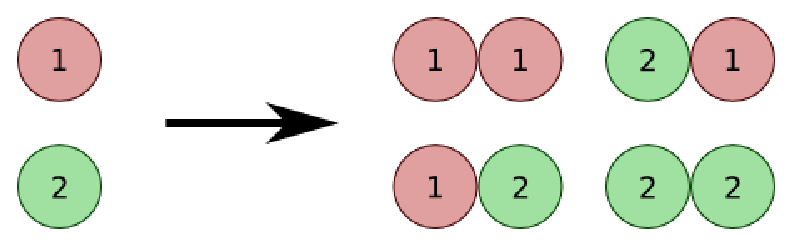
\includegraphics[height=1.91cm]{Figures/4Chapter/sequences}
\end{center}
\end{example}

\begin{example}
The power set of $S$, denoted by $2^S$, is the set of all subsets of $S$.
In set theory, $2^S$ represents the set of all functions from $S$ to $\{ 0, 1\}$.
By identifying a function in $2^S$ with the corresponding preimage of one, we obtain a bijection between $2^S$ and the subsets of $S$.
In particular, each function in $2^S$ is the characteristic function of a subset of $S$.

Suppose that $S$ is finite with $n = |S|$ elements.
For every element of $S$, a characteristic function in $2^S$ is either zero or one.
There are therefore $2^n$ distinct characteristic functions from $S$ to $\{ 0, 1\}$.
Hence, the number of distinct subsets of $S$ is given by $2^n$.

\begin{center}
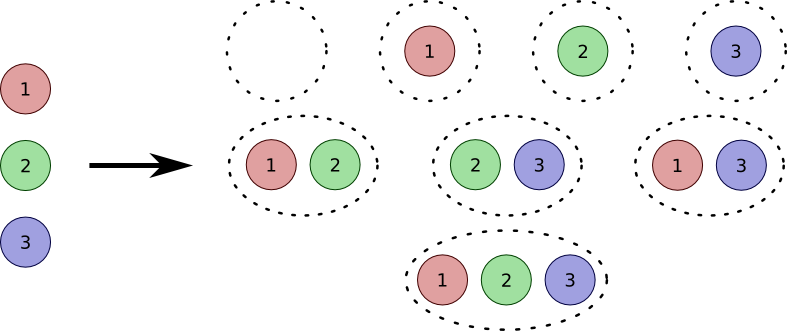
\includegraphics[height=4.965cm]{Figures/4Chapter/powerset}
\end{center}
\end{example}


\section{Permutations}

Again, consider the integer set $S = \{ 1, 2, \ldots, n \}$.
A \emph{permutation} of $S$ is an ordered arrangement of its elements, a list without repetitions. \index{Permutation}
The number of permutations of $S$ can be computed as follows.
First, there are $n$ distinct possibilities for the first item in the list.
The number of possibilities for the second item is $n-1$, namely all the integers in $S$ except the first element in the list.
Similarly, the number of distinct possibilities for the $m$th item is $n - m + 1$.
This pattern continues until all the elements in $S$ are recorded.
Summarizing, we find that the total number of permutations of $S$ is $n$ \emph{factorial}, \index{Factorial}
\begin{equation*}
n! = n (n-1) \cdots 1 .
\end{equation*}

\begin{example}
We wish to compute the number of permutations of $S = \{ 1, 2, 3 \}$.
Since the set $S$ possesses three elements, it has $3! = 6$ different permutations.
They can be written as $123, 132, 213, 231, 312, 321$.
\end{example}

\begin{center}
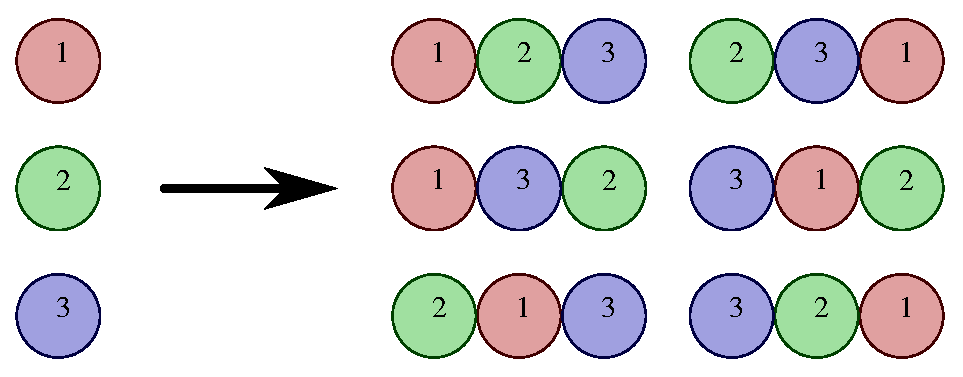
\includegraphics[height=3.06cm]{Figures/4Chapter/permutation}
\end{center}


\subsection{Stirling's Formula*}

The number $n!$ grows very rapidly as a function of $n$.
A good approximation for $n!$ when $n$ is large is given by \emph{Stirling's formula}, \index{Stirling's Formula}
\begin{equation*}
n! \sim n^n e^{-n} \sqrt{ 2 \pi n}
\end{equation*}
as $n \rightarrow \infty$.
The notation $a_n \sim b_n$ signifies that the ratio $a_n / b_n \rightarrow 1$ as $n \rightarrow \infty$.


\subsection{$k$-Permutations}

Suppose that we rank only $k$ elements out of the set $S = \{ 1, 2, \ldots, n \}$, where $k \leq n$.
We wish to count the number of distinct $k$-permutations of $S$.
Following our previous argument, we can choose one of $n$ elements to be the first item listed, one of $(n-1)$ elements for the second item, and so on.
The procedure terminates when $k$ items have been recorded.
The number of possible sequences is then given by
\begin{equation*}
\frac{n!}{(n-k)!} = n (n-1) \cdots (n-k+1) .
\end{equation*}

\begin{example}
A recently formed music group has four original songs they can play.
They are asked to perform two songs at a music festival.
We wish to compute the number of song arrangements the group can offer in concert.
Abstractly, this is equivalent to computing the number of $2$-permutations of four songs.
Thus, the number of distinct arrangements is ${4!}/{2!} = 12$.
\end{example}

\begin{center}
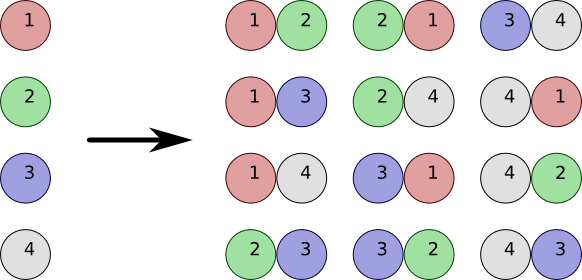
\includegraphics[height=4.215cm]{Figures/4Chapter/kpermutation}
\end{center}

\begin{example}[Sampling without Replacement, with  Ordering]
An urn contains $n$ balls numbered one through $n$.
A ball is picked from the urn, and its number is recorded on an ordered list.
The ball is not replaced in the urn.
This procedure is repeated until $k$ balls are selected from the urn, where $k \leq n$.
We wish to compute the number of possible sequences that results from this experiment.
The number of possibilities is equivalent to the number of $k$-permutations of $n$ elements, which is given by $n! / (n-k)!$.
\end{example}


\section{Combinations}

Consider the integer set $S = \{ 1, 2, \ldots, n \}$.
A \emph{combination} is a subset of $S$. \index{Combination}
We emphasize that a combination differs from a permutation in that elements in a combination have no specific ordering.
The $2$-element subsets of $S = \{ 1, 2, 3, 4 \}$ are
\begin{equation*}
\{ 1, 2 \}, \{ 1, 3 \}, \{ 1, 4 \}, \{ 2, 3 \}, \{ 2, 4 \}, \{ 3, 4 \} ,
\end{equation*}
whereas the $2$-permutations of $S$ are more numerous with
\begin{equation*}
\begin{split}
&( 1, 2 ), ( 1, 3 ), ( 1, 4 ), ( 2, 1 ), ( 2, 3 ), ( 2, 4 ), \\
&( 3, 1 ), ( 3, 2 ), ( 3, 4 ), ( 4, 1 ), ( 4, 2 ), ( 4, 3 ) .
\end{split}
\end{equation*}
There are therefore fewer $2$-element subsets of $S$ than $2$-permutations of $S$.

\begin{center}
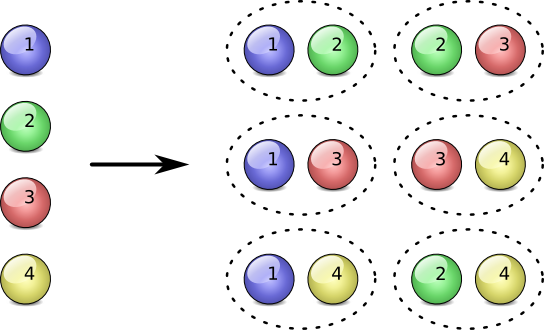
\includegraphics[height=4.95cm]{Figures/4Chapter/combination}
\end{center}

We can compute the number of $k$-element combinations of $S = \{ 1, 2, \ldots, n \}$ as follows.
First, we note that a $k$-permutation can be formed by first selecting $k$ objects from $S$ and then ordering them.
There are $k!$ distinct ways of ordering $k$ objects.
The number of $k$-permutations must then equal the number of $k$-element combinations multiplied by $k!$.
Since the total number of $k$-permutations of $S$ is $n! / (n-k)!$, the number of $k$-element combinations is found to be
\begin{equation*}
\binom{n}{k} = \frac{n!}{k! (n-k)!} = \frac{ n (n-1) \cdots (n-k+1) }{ k! } .
\end{equation*}
This expression is termed a \emph{binomial coefficient}. \index{Binomial Coefficient}
Observe that selecting a $k$-element subset of $S$ is equivalent to choosing the $n-k$ elements that belong to its complement.
It follows that
\begin{equation*}
\binom{n}{k} = \binom{n}{n-k} .
\end{equation*}

\begin{example}[Sampling without Replacement or Ordering]
An urn contains $n$ balls numbered one through $n$.
A ball is drawn from the urn and placed in a separate jar.
This process is repeated until the jar contains $k$ balls, where $k \leq n$.
We wish to compute the number of distinct combinations the jar can hold after the completion of this experiment.
Because there is no ordering in the jar, this amounts to counting the number of $k$-element subsets of a given $n$-element set, which is given by
\begin{equation*}
\binom{n}{k} = \frac{n!}{k! (n-k)!}.
\end{equation*}
\end{example}

Again, let $S = \{1, 2, \ldots, n\}$.
Since a combination is also a subset and the number of $k$-element combinations of $S$ is $\binom{n}{k}$, the sum of the binomial coefficients $\binom{n}{k}$ over all values of $k$ must be equal to the number of elements in the power set of $S$.
Thus, we get
\begin{equation*}
\sum_{k=0}^n \binom{n}{k} = 2^n .
\end{equation*}


\section{Partitions}

Abstractly, a combination is equivalent to partitioning a set into two subsets, one containing $k$ objects and the other containing the $n-k$ remaining objects.
In general, the set $S = \{ 1, 2, \ldots, n \}$ can be partitioned into $r$ subsets.
Let $n_1, n_2, \ldots, n_r$ be nonnegative integers such that
\begin{equation*}
\sum_{p = 1}^r n_p = n.
\end{equation*}
Consider the following iterative algorithm that leads to a \emph{partition} of $S$. \index{Partition}
First, we choose a subset of $n_1$ elements from $S$.
Having selected the first subset, we pick a second subset containing $n_2$ elements from the remaining $n - n_1$ elements.
We continue this procedure by successively choosing subsets of $n_p$ elements from the remaining $n - n_1 - \cdots - n_{p-1}$ elements, until no element remains.
This algorithm yields a partition of $S$ into $r$ subsets, with the $p$th subset containing exactly $n_p$ elements.

We wish to count the number of such partitions.
We know that there are $\binom{n}{n_1}$ ways to form the first subset.
Examining our algorithm, we see that there are exactly
\begin{equation*}
\binom{n - n_1 - \cdots - n_{p-1}}{n_p}
\end{equation*}
ways to form the $p$th subset.
Using the counting principle, the total number of partitions is then given by
\begin{equation*}
\binom{n}{n_1} \binom{n - n_1}{n_2}
\cdots \binom{n - n_1 - \cdots - n_{r-1}}{n_r},
\end{equation*}
which after simplification can be written as
\begin{equation*}
\binom{n}{n_1, n_2, \ldots, n_r}
= \frac{n!}{n_1! n_2! \cdots n_r!} .
\end{equation*}
This expression is called a \emph{multinomial coefficient}. \index{Multinomial coefficient}

\begin{example}
A die is rolled nine times.
We wish to compute the number of outcomes for which every odd number appears three times.
The number of distinct sequences in which one, three, and five each appear three times is equal to the number of partitions of $\{ 1, 2, \ldots, 9 \}$ into three subsets of size three, namely
\begin{equation*}
\frac{9!}{3! 3! 3!} = 1680 .
\end{equation*}
\end{example}

In the above analysis, we assume that the cardinality of each subset is fixed.
Suppose instead that we are interested in counting the number of ways to pick the cardinality of the subsets that form the partition. \index{Partition}
Specifically, we wish to compute the number of ways integers $n_1, n_2, \ldots, n_r$ can be selected such that every integer is nonnegative and
\begin{equation*}
\sum_{p = 1}^r n_p = n.
\end{equation*}
We can visualize the number of possible assignments as follows.
Picture $n$ balls space out on a straight line and consider $r-1$ vertical markers, each of which can be put between two consecutive balls, before the first ball, or after the last ball. 
For instance, if there are five balls and two markers then one possible assignment is illustrated below.

\begin{center}
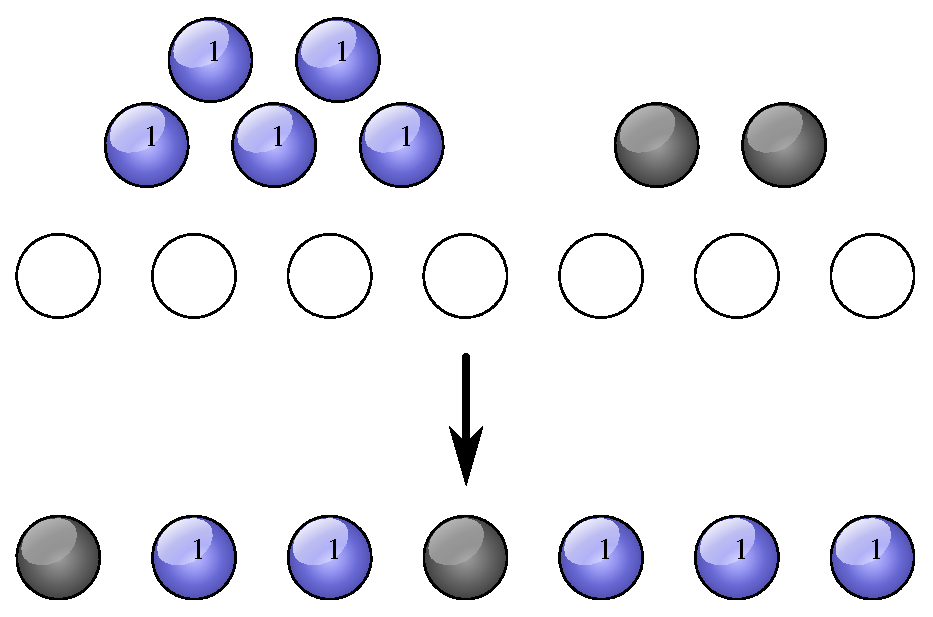
\includegraphics[height=5.28cm]{Figures/4Chapter/partitioning}
\end{center}

The number of objects in the first subset corresponds to the number balls before the first marker.
Similarly, the number of objects in the $p$th subset is equal to the number of balls between the $p$th marker and the preceding one.
Finally, the number of objects in the last subset is simply the number of balls after the last marker.
The integer assignment associated with the figure above is
\begin{equation*}
(n_1, n_2, n_3) = (0,2,3).
\end{equation*}

\begin{center}
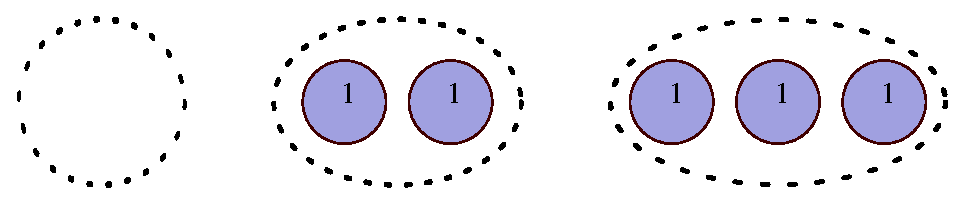
\includegraphics[height=1.53cm]{Figures/4Chapter/partitioning2}
\end{center}

In this scheme, two consecutive markers imply that the corresponding subset is empty.
There is a natural bijection between an integer assignment and the graphical representation depicted above.
To count the number of possible integer assignments, it suffices to calculate the number of ways to position the markers and the balls.
In particular, there are $n + r - 1$ positions, $n$ balls and $r - 1$ markers.
The number of ways to assign the markers is equal to the number of $n$-combinations of $n + r - 1$ elements,
\begin{equation*}
\binom{n + r - 1}{n} = \binom{n + r - 1}{r - 1} .
\end{equation*}

\begin{example}[Sampling with Replacement, without Ordering]
An urn contains $r$ balls numbered one through $r$.
A ball is drawn from the urn and its number is recorded.
The ball is then returned to the urn.
This procedure is repeated a total of $n$ times.
The outcome of this experiment is a table that contains the number of times each ball has come in sight.
We are interested in computing the number of distinct outcomes.
This is equivalent to counting the ways a set with $n$ elements can be partitioned into $r$ subsets.
The number of possible outcomes is therefore given by
\begin{equation*}
\binom{n + r - 1}{n} = \binom{n + r - 1}{r - 1} .
\end{equation*}
\end{example}


\section{Computing Probabilities}

In this section, we present two applications of combinatorics to computing the probability of winning the lottery.

\begin{example}[Pick 3 Texas Lottery]
The Texas Lottery game ``Pick $3$'' is easy to play.
A player must pick three numbers from zero to nine, and choose how to play them: exact order or any order.
The Pick $3$ balls are drawn using three air-driven machines.
These machines use compressed air to mix and select each ball.

The probability of winning while playing the exact order is
\begin{equation*}
\frac{1}{10} \frac{1}{10} \frac{1}{10}
= \frac{1}{1000} .
\end{equation*}
The probability of winning while playing any order depends on the numbers selected.
If three distinct numbers are selected then the probability of winning is
\begin{equation*}
\frac{3!}{1000} = \frac{3}{500} .
\end{equation*}
If a number is repeated twice, the probability of winning is
\begin{equation*}
\frac{\binom{3}{2}}{1000} = \frac{3}{1000} .
\end{equation*}
While, if the same number is selected three times, the probability of winning becomes $1/1000$.
\end{example}

\begin{example}[Mega Millions Texas Lottery]
To play the Mega Millions game, a player must select five numbers from $1$ to $56$ in the upper white play area of the play board, and one Mega Ball number from $1$ to $46$ in the lower yellow play area of the play board.
All drawing equipment is stored in a secured on-site storage room.
Only authorized drawings department personnel have keys to the door.
Upon entry of the secured room to begin the drawing process, a lottery drawing specialist examines the security seal to determine if any unauthorized access has occurred.
For each drawing, the Lotto Texas balls are mixed by four acrylic mixing paddles rotating clockwise.
High speed is used for mixing and low speed for ball selection.
As each ball is selected, it rolls down a chute into an official number display area.
We wish to compute the probability of winning the Mega Millions Grand Prize, which require the correct selection of the five white balls plus the gold Mega ball.

The probability of winning the Mega Millions Grand Prize is
\begin{equation*}
\frac{1}{\binom{56}{5}} \frac{1}{46}
= \frac{51!5!}{56!} \frac{1}{46}
= \frac{1}{175 711 536} .
\end{equation*}
\end{example}


\chapter{Discrete Random Variables}
\label{chapter:DiscreteRandomVariables}

Suppose that an experiment and a sample space are given.
A \emph{random variable} is a real-valued function of the outcome of the experiment. \index{Random variable}
In other words, the random variable assigns a specific number to every possible outcome of the experiment.
The numerical value of a particular outcome is simply called the \emph{value} of the random variable. \index{Value of a random variable}
Because of the structure of real numbers, it is possible to define pertinent statistical properties on random variables that otherwise do not apply to probability spaces in general.

\begin{figure}[ht]
\begin{center}
\begin{psfrags}
\psfrag{S}[l]{Sample Space}
\psfrag{1}[c]{$1$}
\psfrag{2}[c]{$2$}
\psfrag{3}[c]{$3$}
\psfrag{4}[c]{$4$}
\psfrag{5}[c]{$5$}
\psfrag{6}[c]{$6$}
\psfrag{7}[c]{$7$}
\psfrag{R}[r]{Real Numbers}
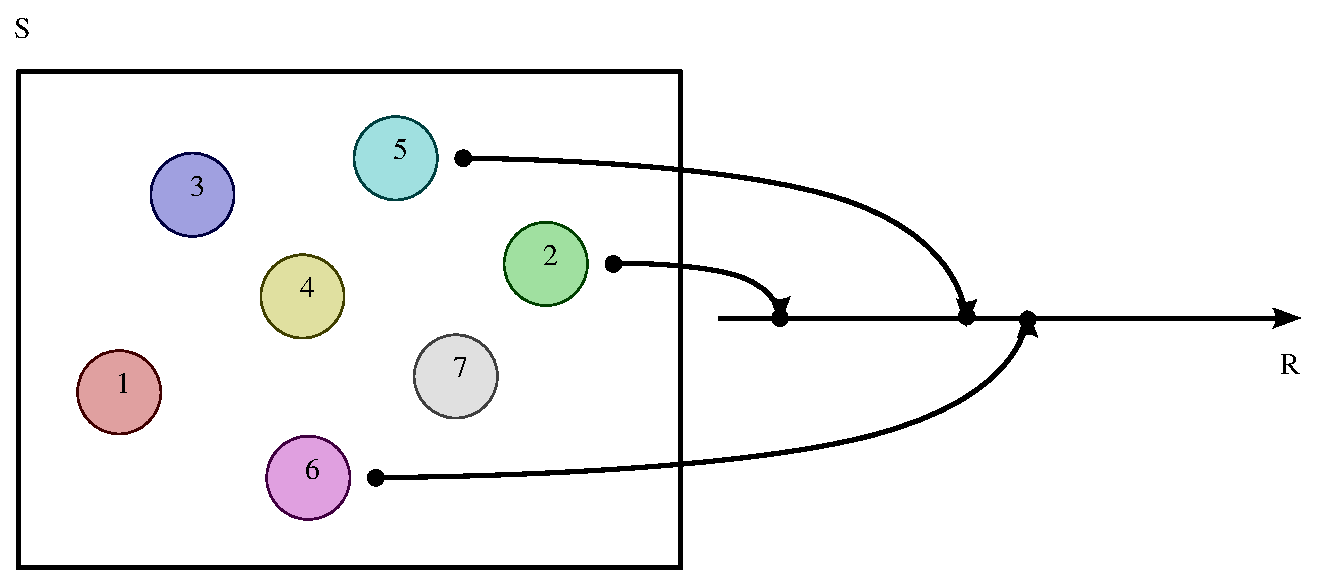
\includegraphics[height=4.96cm]{Figures/5Chapter/rv}
\caption{The sample space in this example has seven possible outcomes.
A random variable maps each of these outcomes to a real number.}
\end{psfrags}
\end{center}
\end{figure}

\begin{example}
There are six possible outcomes to the rolling of a fair die, namely each of the six faces.
These faces map naturally to the integers one through six.
The value of the random variable, in this case, is simply the number of dots that appear on the top face of the die.

\begin{figure}[ht]
\begin{center}
\begin{psfrags}
\psfrag{1}[c]{$1$}
\psfrag{2}[c]{$2$}
\psfrag{3}[c]{$3$}
\psfrag{4}[c]{$4$}
\psfrag{5}[c]{$5$}
\psfrag{6}[c]{$6$}
\includegraphics[height=5.99cm]{Figures/5chapter/rvdices}
\caption{This random variable takes its input from the rolling of a die and assigns to each outcome a real number that corresponds to the number of dots that appear on the top face of the die.}
\end{psfrags}
\end{center}
\end{figure}
\end{example}

The simplest class of random variables is the collection of \emph{discrete random variables}. \index{Discrete random variable}
A variable is called discrete if its range is finite or countably infinite; that is, if the random variable can only take a finite or countable number of values.

\begin{example}
Consider the experiment where a coin is tossed repetitively until heads is observed.
The corresponding function, which maps the number of tosses to an integer, is a discrete random variable that takes a countable number of values.
The range of this random variable is given by the positive integers $\{1, 2, \ldots \}$.
\end{example}

\section{Probability Mass Functions}

A discrete random variable $X$ is characterized by the probability of each of the elements in the range of $X$.
We identify the probabilities of individual elements in the range of $X$ using the \emph{probability mass function (PMF)} of $X$, which we denote by $p_X$. \index{Probability mass function (PMF)}
If $x$ is a possible value of $X$ then the \emph{probability mass} of $x$, written $p_X (x)$, is defined by
\begin{equation} \label{equation:PMF}
p_X (x) = \Pr ( \{ X = x \} ) = \Pr ( X = x ) .
\end{equation}
Equivalently, we can think of $p_X (x)$ as the probability of the set of all outcomes in $\Omega$ for which $X$ is equal to $x$,
\begin{equation*}
p_X (x)
= \Pr (  X^{-1} (x)  )
= \Pr ( \{ \omega \in \Omega | X(\omega) = x \} ) .
\end{equation*}

\begin{figure}[ht]
\begin{center}
\begin{psfrags}
\psfrag{S}[l]{Sample Space}
\psfrag{1}[c]{$1$}
\psfrag{2}[c]{$2$}
\psfrag{3}[c]{$3$}
\psfrag{4}[c]{$4$}
\psfrag{5}[c]{$5$}
\psfrag{6}[c]{$6$}
\psfrag{7}[c]{$7$}
\psfrag{x}[l]{$x$}
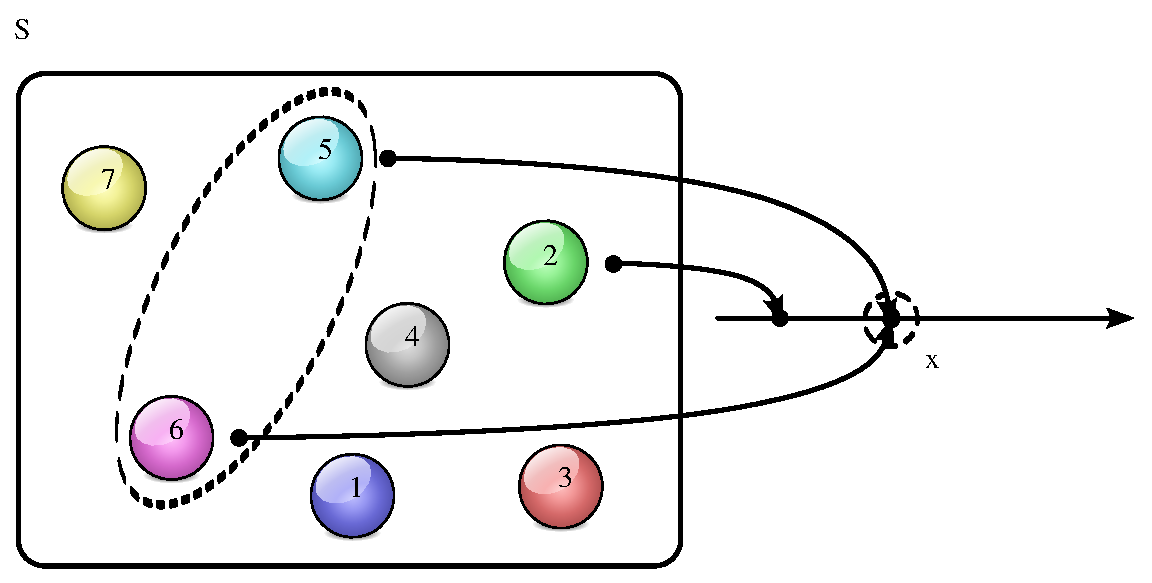
\includegraphics[height=4.97cm]{Figures/5Chapter/pmf}
\caption{The probability mass of $x$ is given by the probability of the set of all outcomes which $X$ maps to $x$.}
\end{psfrags}
\end{center}
\end{figure}


Let $X(\Omega)$ denote the collection of all the possible numerical values $X$ can take; this set is known as the range of $X$.
Using this notation, we can write
\begin{equation} \label{equation:NormalizationPMF}
\sum_{x \in X(\Omega)} p_X(x) = 1 .
\end{equation}
We emphasize that the sets defined by $\{ \omega \in \Omega | X(\omega) = x \}$ are disjoint and form a partition of the sample space $\Omega$, as $x$ ranges over all the possible values in $X (\Omega)$.
Thus, \eqref{equation:NormalizationPMF} follows immediately from the countable additivity axiom and the normalization axiom of probability laws.
In general, if $X$ is a discrete random variable and $S$ is a subset of $X(\Omega)$, we can write
\begin{equation} \label{equation:FunctionPMF}
\Pr (S) = \Pr \left( \{ \omega \in \Omega | X(\omega) \in S \} \right) = \sum_{x \in S} p_X (x) .
\end{equation}
This equation offers an explicit formula to compute the probability of any subset of $X (\Omega)$, provided that $X$ is discrete.

\begin{example}
An urn contains three balls numbered one, two and three.
Two balls are drawn from the urn without replacement.
We wish to find the probability that the sum of the two selected numbers is odd.

Let $\Omega$ be the set of ordered pairs corresponding to the possible outcomes of the experiment,
$\Omega = \{ (1, 2), (1, 3), (2, 1), (2, 3), (3, 1), (3, 2) \}$.
Note that these outcomes are equiprobable.
We employ $X$ to represent the sum of the two selected numbers.
The PMF of random variable $X$ is given by
\begin{equation*}
p_X (3) = p_X (4) = p_X (5) = \frac{1}{3}.
\end{equation*}
If $S$ denotes the event that the sum of the two numbers is odd, then the probability of the sum being odd can be computed as follows,
\begin{equation*}
\Pr (S) = \Pr ( \{ 3, 5 \} )
= p_X (3) + p_X (5) = \frac{2}{3} .
\end{equation*}
\end{example}


\section{Important Discrete Random Variables}

A number of discrete random variables appears frequently in problems related to probability.
These random variables arise in many different contexts, and they are worth getting acquainted with.
In general, discrete random variables occur primarily in situations where counting is involved.


\subsection{Bernoulli Random Variables}

The first and simplest discrete random variable is the \emph{Bernoulli random variable}. \index{Bernoulli random variable}
Let $X$ be a random variable that takes on only two possible numerical values, $X(\Omega) = \{0, 1\}$.
Then $X$ is a Bernoulli random variable and its PMF is given by
\begin{equation*}
p_X (x) = \left\{ \begin{array}{ll}
1 - p, & \text{if }x = 0 \\
p, & \text{if }x = 1
\end{array} \right.
\end{equation*}
where $p \in [0, 1]$.

\begin{figure}[ht]
\begin{center}
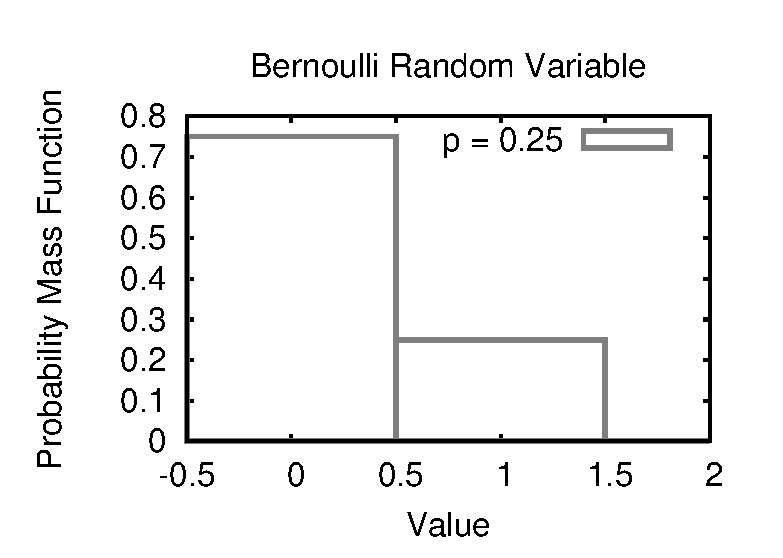
\includegraphics[width=8.5cm]{Figures/5chapter/bernoulli_pmf}
\end{center}
\caption{The PMF of a Bernoulli random variable appears above for parameter $p = 0.25$.}
\end{figure}

\begin{example}
Consider the flipping of a biased coin, for which heads is obtained with probability $p$ and tails is obtained with probability $1-p$.
A random variable that maps heads to one and tails to zero is a Bernoulli random variable with parameter~$p$.
In fact, every Bernoulli random variable is equivalent to the tossing of a coin.
\end{example}


\subsection{Binomial Random Variables}
\label{subsection:BinormialRandomVariables}

Multiple independent Bernoulli random variables can be combined to construct more sophisticated random variables.
Suppose $X$ is the sum of $n$ independent and identically distributed Bernoulli random variables.
Then $X$ is called a \emph{binomial random variable} with parameters $n$ and $p$. \index{Binomial random variable}
The PMF of $X$ is given by
\begin{equation*}
p_X (k) = \Pr (X = k)
= \binom{n}{k} p^k (1-p)^{n-k},
\end{equation*}
where $k = 0, 1, \ldots n$.
Note that we can easily verify that $X$ fulfills the normalization axiom,
\begin{equation*}
\sum_{k=0}^n \binom{n}{k} p^k (1-p)^{n-k}
= \left( p + (1-p) \right)^n = 1.
\end{equation*}

\begin{figure}[ht]
\begin{center}
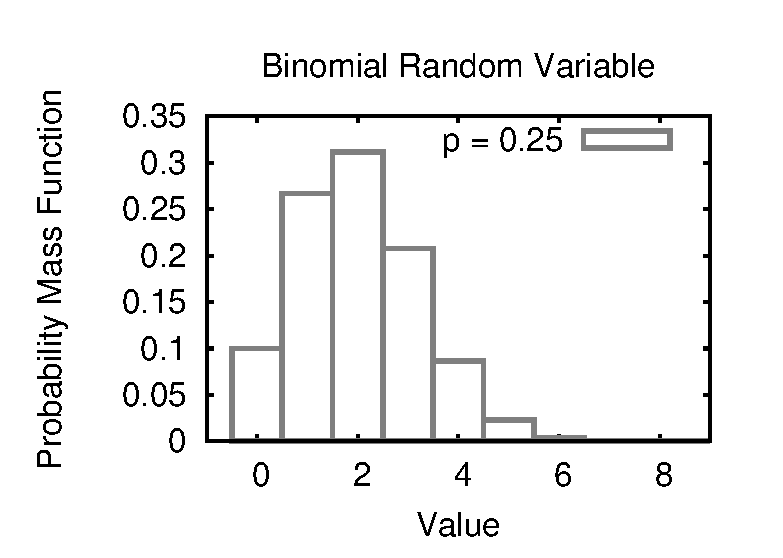
\includegraphics[width=8.5cm]{Figures/5chapter/binomial_pmf}
\end{center}
\caption{This figure shows a binomial random variable with parameters $n = 8$ and $p = 0.25$.}
\end{figure}

\begin{example} \label{BrazosSodaCompany1}
The Brazos Soda Company creates an ``Under the Caps'' promotion whereby a customer can win an instant cash prize of \$10 by looking under a bottle cap.
The likelihood to win is one in twelve, and it is independent from bottle to bottle.
A customer buys twelve bottles of soda from this company.
We wish to find the PMF of the number of winning bottles, which we denote by $X$.
Also, we want to compute the probability of winning more than \$40.

The random variable $X$ is binomial with parameters $n = 12$ and $p = 1/12$.
Its PMF is given by
\begin{equation*}
p_X (k) = \binom{12}{k} \left( \frac{1}{12} \right)^k
\left( \frac{11}{12} \right)^{n-k}
= \binom{12}{k} \frac{11^{n-k}}{12^n} ,
\end{equation*}
where $k = 0, 1, \ldots, 12$.
The probability of winning more than \$40 is
\begin{equation*}
\Pr (\$10 \times X > \$40)
= \Pr (X > 4)
= \sum_{k=5}^{12} \binom{12}{k} \frac{11^{n-k}}{12^n} .
\end{equation*}
\end{example}


\subsection{Poisson Random Variables}

The probability mass function of a \emph{Poisson random variable} is given by \index{Poisson random variable}
\begin{equation*}
p_X (k) = \frac{\lambda^k}{k!} e^{- \lambda}, \quad k = 0, 1, \ldots
\end{equation*}
where $\lambda$ is a positive number.
Note that, using Taylor series expansion,  we have
\begin{equation*}
\sum_{k = 0}^{\infty} p_X (k)
= \sum_{k = 0}^{\infty} \frac{\lambda^k}{k!} e^{- \lambda}
= e^{- \lambda} \sum_{k = 0}^{\infty} \frac{\lambda^k}{k!}
= e^{- \lambda} e^{\lambda} = 1 ,
\end{equation*}
which shows that this PMF fulfills the normalization axiom of probability laws.
The Poisson random variable is of fundamental importance when counting the number of occurrences of a phenomenon in a certain time period.
It finds extensive use in networking, inventory management and queueing applications.

\begin{figure}[ht]
\begin{center}
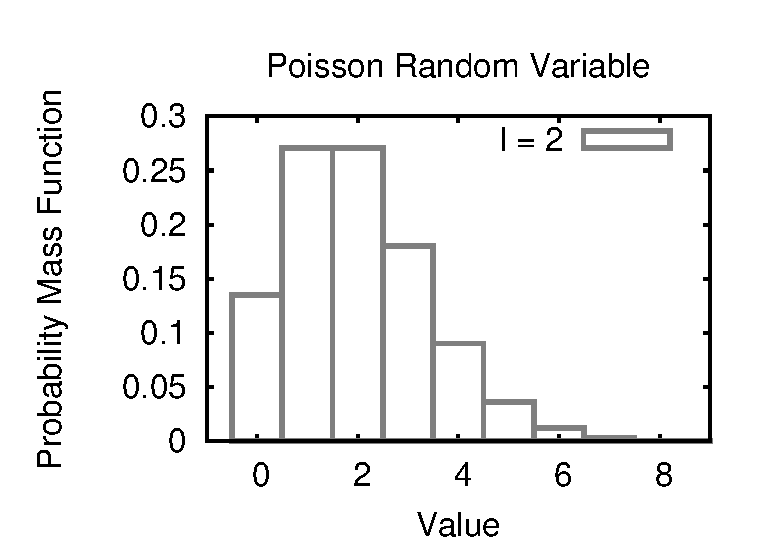
\includegraphics[width=8.5cm]{Figures/5chapter/poisson_pmf}
\caption{This figure shows the PMF of a Poisson random variable with parameter $\lambda = 2$.  Note that the values of the PMF are only present for $k = 0, 1, \ldots, 8$.}
\end{center}
\end{figure}

\begin{example}
Requests at an Internet server arrive at a rate of $\lambda$ connections per second.
The number of service requests per second is modeled as a random variable with a Poisson distribution.
We wish to find the probability that no service requests arrive during a time interval of one second.

Let $N$ be a random variable that represents the number of requests that arrives within a span of one second.
By assumption, $N$ is a Poisson random variable with PMF
\begin{equation*}
p_N (k) = \frac{ \lambda^k }{k!} e^{-\lambda} .
\end{equation*}
The probability that no service requests arrive in one second is simply given by $p_N (0) = e^{-\lambda}$.
\end{example}

It is possible to obtain a Poisson random variable as the limit of a sequence of binomial random variables.
Fix $\lambda$ and let $p_n = \lambda/n$.
For $k = 1, 2, \ldots n$, we define the PMF of the random variable $X_n$ as
\begin{equation*}
\begin{split}
p_{X_n} (k) &= \Pr (X_n = k)
= \binom{n}{k} p_n^k (1-p_n)^{n-k} \\
&= \frac{n!}{k!(n-k)!} \left( \frac{\lambda}{n} \right)^k
\left( 1 - \frac{\lambda}{n} \right)^{n-k} \\
&= \frac{n!}{n^k (n-k)!} \frac{\lambda^k}{k!}
\left( 1 - \frac{\lambda}{n} \right)^{n-k} .
\end{split}
\end{equation*}
In the limit, as $n$ approaches infinity, we get
\begin{equation*}
\lim_{n \rightarrow \infty} p_{X_n} (k)
= \lim_{n \rightarrow \infty} \frac{n!}{n^k (n-k)!} \frac{\lambda^k}{k!}
\left( 1 - \frac{\lambda}{n} \right)^{n-k}
= \frac{\lambda^k}{k!} e^{- \lambda} .
\end{equation*}
Thus, the sequence of binomial random variables $\{ X_n \}$ converges in distribution to the Poisson random variable $X$.

\begin{figure}[ht]
\begin{center}
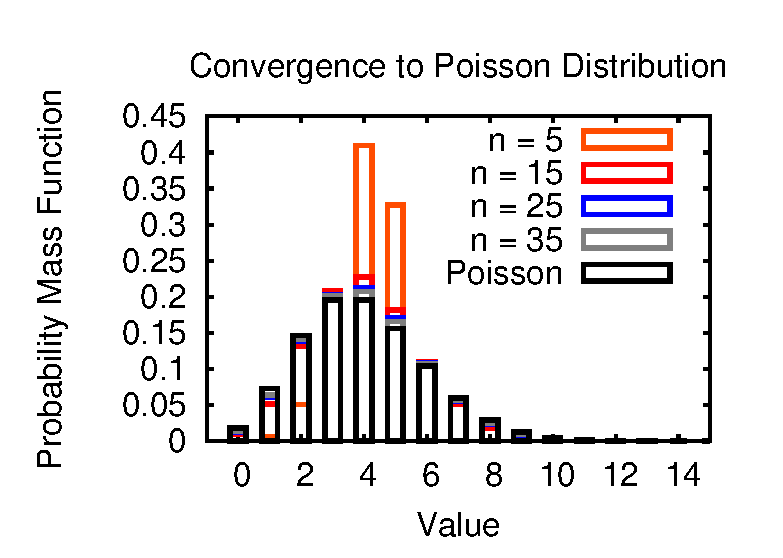
\includegraphics[width=8.5cm]{Figures/5chapter/convergence_pmf}
\end{center}
\caption{The levels of a binomial PMF with parameter $p = \lambda/n$ converge to the probabilities of a Poisson PMF with parameter $\lambda$ as $n$ increases to infinity.}
\end{figure}

This discussion suggests that the Poisson PMF can be employed to approximate the PMF of a binomial random variable in certain circumstances.
Suppose that $Y$ is a binomial random variable with parameters $n$ and $p$.
If $n$ is large and $p$ is small then the probability that $Y$ equals $k$ can be approximated by
\begin{equation*}
p_{Y} (k) = \frac{n!}{n^k (n-k)!} \frac{\lambda^k}{k!}
\left( 1 - \frac{\lambda}{n} \right)^{n-k}
\approx \frac{\lambda^k}{k!} e^{- \lambda} ,
\end{equation*}
where $\lambda = n p$.
The latter expression can be computed numerically in a straightforward manner.

\begin{example}
The probability of a bit error on a wireless communication channel is equal to $10^{-2}$.
We wish to approximate the probability that a block of $1000$ bits has four or more errors.

Assume that the probability of individual errors is independent from bit to bit.
The transmission of each bit can be modeled as a Bernoulli trial, with a zero indicating a correct transmission and a one representing a bit error.
The total number of bit errors in $1000$ transmissions then corresponds to a binomial random variable with parameters $n = 1000$ and $p = 10^{-2}$.
The probability of making four or more errors can be approximated using a Poisson random variable with constant $\lambda = np = 10$.
Thus, we can approximate the probability that a block of $1000$ bits has four or more errors by
\begin{equation*}
\begin{split}
\Pr [ N \geq 4 ] &= 1 - \Pr [ N < 4 ]
\approx 1 - \sum_{k=0}^3 \frac{\lambda^k}{k!} e^{-\lambda} \\
&= 1 - e^{-10} \left( 1 + 10 + 50 + \frac{500}{3} \right) \\
&\approx 0.01034 .
\end{split}
\end{equation*}
% The exact value in this case is
\end{example}


\subsection{Geometric Random Variables}

Consider a random experiment where a Bernoulli trial is repeated multiple times until a one is observed.
At each time step, the probability of getting a one is equal to $p$ and the probability of getting a zero is $1-p$.
The number of trials carried out before completion, which we denote by $X$, is recorded as the outcome of the experiment.
The random variable $X$ is a \emph{geometric random variable}, and its PMF is given by \index{Geometric random variable}
\begin{equation*}
p_X (k) = (1-p)^{k-1} p, \quad k = 1, 2, \ldots
\end{equation*}
We stress that $(1-p)^{k-1} p$ simply represents the probability of obtaining a sequence of $k-1$ zero immediately followed by a one.

\begin{figure}[ht]
\begin{center}
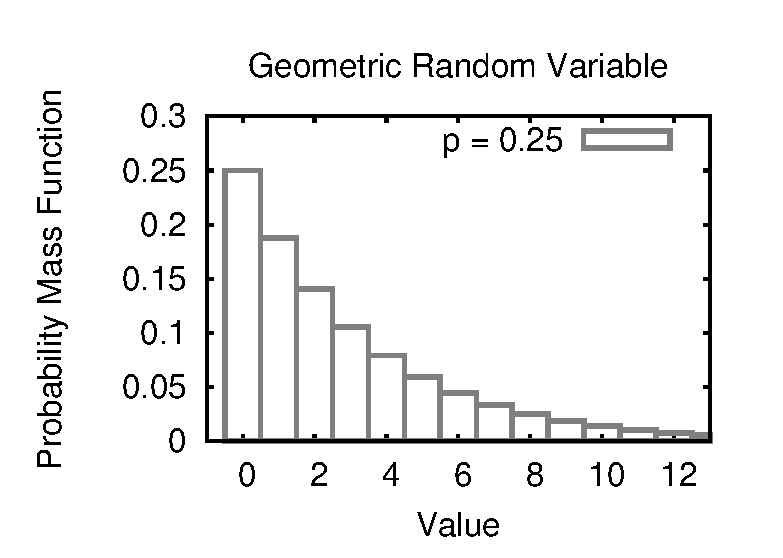
\includegraphics[width=8.5cm]{Figures/5chapter/geometric_pmf}
\end{center}
\caption{The PMF of a geometric random variable is a decreasing function of $k$.
It is plotted above for $p = 0.25$.
The values of the PMF are only present for $k = 1, 2, \ldots, 12$.}
\end{figure}

\begin{example}
The Brazos Soda Company introduces another ``Under the Caps'' promotion.
This time, a customer can win an additional bottle of soda by looking under the cap of her bottle.
The probability to win is $1/5$, and it is independent from bottle to bottle.
A customer purchases one bottle of soda from the Brazos Soda company and hence enters the contest.
For every extra bottle of soda won by looking under the cap, the customer gets an additional chance to play.
We wish to find the PMF of the number of bottles obtained by this customer.

Let $X$ denote the total number of bottles obtained by this customer.
The random variable $X$ is geometric and its PMF is
\begin{equation*}
p_X (k) = \left( \frac{1}{5} \right)^{k-1} \frac{4}{5},
\end{equation*}
where $k = 1, 2, \ldots$
\end{example}

\paragraph{Memoryless Property:}
A remarkable aspect of the geometric random variable is that it satisfies the \emph{memoryless property}, \index{Memoryless property}
\begin{equation*}
\Pr (X = k + j | X > k) = \Pr (X = j).
\end{equation*}
This can be established using the definition of conditional probability.
Let $X$ be a geometric random variable with parameter $p$, and assume that $k$ and $j$ are positive integers.
We can write the conditional probability of $X$ as
\begin{equation*}
\begin{split}
\Pr (X = k + j | X > k)
&= \frac{\Pr( \{ X =  k + j \} \cap \{ X > k \} ) }{ \Pr ( X > k ) } \\
&= \frac{\Pr( X = k + j ) }{ \Pr ( X > k ) }
= \frac{(1 - p)^{k + j - 1} p }{ (1 - p)^k  } \\
&= (1 - p)^{j - 1} p
= \Pr (X = j).
\end{split}
\end{equation*}
In words, the probability that the number of trials carried out before completion is $k + j$, given $k$ unsuccessful trials, is equal to the unconditioned probability that the total number of trials is $j$.
It can be shown that the geometric random variable is the only discrete random variable that possesses the memoryless property.


\subsection{Discrete Uniform Random Variables}

A finite random variable where all the possible outcomes are equally likely is called a \emph{discrete uniform random variable}. \index{Uniform random variable (discrete)}
Let $X$ be a uniform random variable taking value in $X (\Omega) = \{ 1, 2, \ldots, n \}$.
Its PMF is therefore given by
\begin{equation*}
p_X (k) = \left\{ \begin{array}{ll}
1/n, & \text{if }k = 1, 2, \ldots, n \\
0, & \text{otherwise} .
\end{array} \right.
\end{equation*}
We encountered specific cases of this random variable before.
The tossing of a fair coin and the rolling of a die can both be used to construct uniform random variables.

\begin{figure}[ht]
\begin{center}
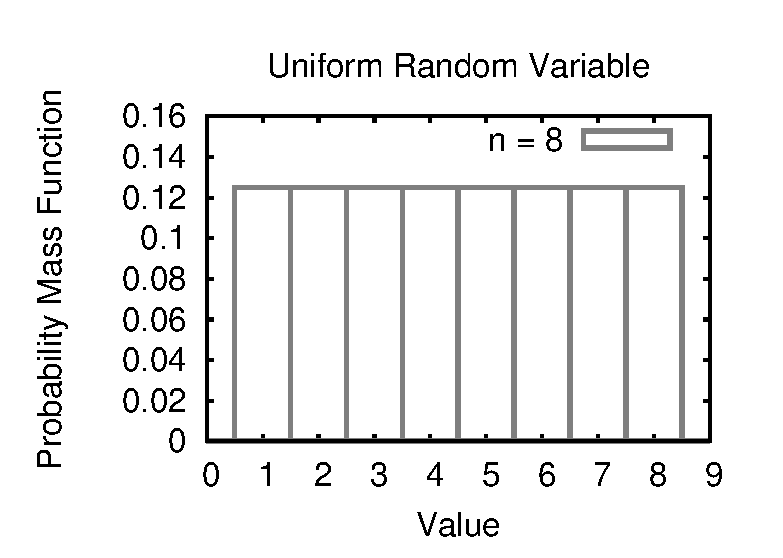
\includegraphics[width=8.5cm]{Figures/5chapter/uniform_pmf}
\end{center}
\caption{A uniform random variable corresponds to a situation where all the possible values of the random variable are equally likely.
It is shown above for the case where $n = 8$.}
\end{figure}


\section{Functions of Random Variables}
\label{subsection:FunctionDiscreteRV}
\index{Functions of Random Variables}

Recall that a random variable is a function of the outcome of an experiment.
Given a random variable $X$, it is possible to create a new random variable $Y$ by applying a real-valued function $g(\cdot)$ to $X$.
If $X$ is a random variable then $Y = g(X)$ is also a random variable since it associates a numerical value to every outcome of the experiment.
In particular, if $\omega \in \Omega$ is the outcome of the experiment, then $X$ takes on value $x = X(\omega)$ and $Y$ takes on value $Y(\omega) = g(x)$.

\begin{figure}[htb!]
\begin{center}
\begin{psfrags}
\psfrag{1}[c]{$1$}
\psfrag{2}[c]{$2$}
\psfrag{3}[c]{$3$}
\psfrag{4}[c]{$4$}
\psfrag{5}[c]{$5$}
\psfrag{S}[l]{Sample Space}
\psfrag{X}[c]{$X$}
\psfrag{Y}[c]{$Y = g(X)$}
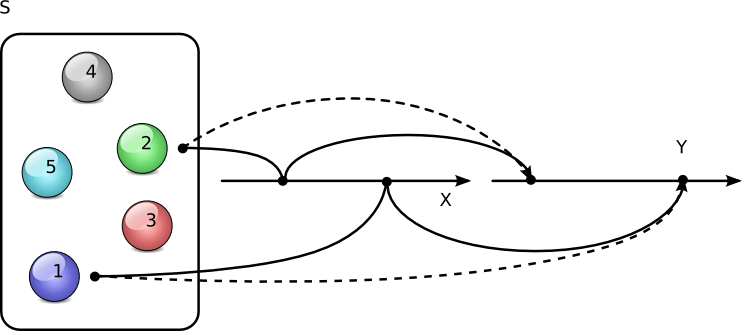
\includegraphics[height=4.97cm]{Figures/5Chapter/fcn}
\end{psfrags}
\caption{A real-valued function of a random variable is a random variable itself.
In this figure, $Y$ is obtained by passing random variable $X$ through a function $g$.}
\end{center}
\end{figure}

Furthermore, if $X$ is a discrete random variable, then so is $Y$.
The set of all the possible values $Y$ can take is denoted by $g(X(\Omega))$, and the number of elements in $g(X(\Omega))$ is no greater than the number of elements in $X(\Omega)$.
The PMF of $Y$, which we represent by $p_Y (y)$, is obtained as follows.
If $y \in g(X(\Omega))$ then
\begin{equation} \label{equation:DefinitionFunctionPMF}
p_Y (y) = \sum_{ \{x \in X(\Omega) | g(x) = y \} } p_X (x) ;
\end{equation}
otherwise, $p_Y (y) = 0$.
In particular, $p_Y (y)$ is non-zero only if there exists an $x \in X(\Omega)$ such that $g(x) = y$ and $p_X (x) > 0$.

\begin{example}
Let $X$ be a random variable and let $Y = g(X) = aX + b$, where $a$ and $b$ are constant.
That is, $Y$ is an affine function of $X$.
Suppose that $a \neq 0$, then the probability of $Y$ being equal to value $y$ is given by
\begin{equation*}
p_Y(y) = p_X \left( \frac{ y - b }{a} \right) .
\end{equation*}
\end{example}

Linear and affine functions of random variables are commonplace in probability.
In Example~\ref{BrazosSodaCompany1}, for instance, we have implicitly used the linear function $Y = 10 X$ to compute the probability of winning more than \$40.


\section*{Further Reading}

\begin{small}
\begin{enumerate}
\item Ross, S., \emph{A First Course in Probability}, 7th edition, Pearson Prentice Hall,2006: Sections~4.1--4.2, 4.6--4.8.
\item Bertsekas, D.P., and Tsitsiklis, J.N., \emph{Introduction to Probability}, Athena Scientific, 2002: Sections~2.1--2.3.
\end{enumerate}
\end{small}


\chapter{Continuous Random Variables}

In the previous chapter, we introduced discrete random variables and discussed their properties.
Discrete random variables are very useful in many contexts, yet they form only a small subset of the collection of random variables pertinent to probability and engineering.
In this chapter, we consider random variables with a continuous range of possible values; that is, random variables that can take an uncountable number of values.

Continuous random variables are powerful mathematical tools that allow us to pose and solve important engineering problems, which cannot be addressed using discrete models.
While this extra flexibility is useful and desirable, it comes at a certain cost.
A continuous random variable cannot be characterized by a probability mass function.
This difficulty emerges from the limitations of the third axiom of probability laws, which only applies to countable collections of disjoint events.

Below, we provide a definition for continuous random variables.
Furthermore, we extend and apply the concepts and methods introduced in Chapter~\ref{chapter:DiscreteRandomVariables} to the class of continuous random variables.
In particular, we develop a continuous counterpart to the probability mass function.


\section{Cumulative Distribution Functions}

We begin this chapter by introducing a general concept which can be used to bridge our understanding of discrete and continuous random variables.
The \emph{cumulative distribution function} (CDF) of a random variable $X$ is defined as the probability of the event $\{X \leq x \}$,
\begin{equation*}
F_X (x) = \Prob ( \{ X \leq x \} ) = \Prob (X \leq x).
\end{equation*}
In terms of the underlying sample space, the function $F_X (x)$ represents the probability of the set of all outcomes in $\Omega$ for which $X$ is less than or equal to $x$,
\begin{equation*}
F_X (x) = \Prob \left( X^{-1} ( (- \infty, x]) \right)
= \Prob (\{ \omega \in \Omega | X(\omega) \leq x \}).
\end{equation*}
In essence, the CDF is a convenient way to specify the probability of all events of the form $X \in (-\infty, x]$.

Recall that a random variable is a real-valued function.
The CDF of random variable $X$ therefore exists and is well-defined for any $X$.
Furthermore, since the realization of $X$ is a real number, we have
\begin{gather*}
\lim_{x \rightarrow - \infty} F_X (x) = 0 \\
\lim_{x \rightarrow \infty} F_X (x) = 1.
\end{gather*}
Suppose $x_1 < x_2$, then we can write $\{ X \leq x_2 \}$ as the union of the two disjoint sets $\{ X \leq x_1 \}$ and $\{ x_1 < X \leq x_2 \}$.
It follows that
\begin{equation} \label{equation:MonotoneIncreasingCDF}
\begin{split}
F_X (x_2) &= \Prob (X \leq x_2) \\
&= \Prob (X \leq x_1) + \Prob (x_1 < X \leq x_2) \\
&\geq \Prob (X \leq x_1) = F_X (x_1).
\end{split}
\end{equation}
The CDF is a monotone non-decreasing function.
We note from \eqref{equation:MonotoneIncreasingCDF} that the probability of $X$ falling in the interval $(x_1, x_2]$ is
\begin{equation} \label{equation:IntervalCDF}
\Prob (x_1 < X \leq x_2) = F_X (x_2) - F_X (x_1).
\end{equation}

\subsection{Discrete Random Variables}

Suppose that $X$ is a discrete random variable that takes only integer values.
Then the CDF of $X$ is given by
\begin{equation*}
F_X (x) = \sum_{k \leq x} p_X (k),
\end{equation*}
and its PMF can be computed using the formula
\begin{equation*}
p_X (k) = \Prob ( X \leq k) - \Prob (X \leq k -1 ) = F_X (k) - F_X (k-1).
\end{equation*}

\begin{example}
For instance, let $X$ be a geometric random variable with parameter $p$ and PMF
\begin{equation*}
p_X (k) = (1 - p)^{k-1} p \quad k = 1, 2, \ldots 
\end{equation*}
For $x > 0$, its CDF is then given by
\begin{equation*}
F_X (x) = \sum_{k = 1}^{\lfloor x \rfloor} (1 - p)^{k-1} p
= 1 - (1 - p)^{\lfloor x \rfloor} .
\end{equation*}
For integer $k \geq 1$, the PMF of a geometric random variable $X$ is recovered by calculating
\begin{equation*}
\begin{split}
p_X (k) &= F_X (k) - F_X (k-1) \\
&= \left( 1 - (1-p)^k \right) - \left( 1 - (1-p)^{k-1} \right) \\
&= (1 - p)^{k-1} - (1-p) (1-p)^{k-1} \\
&= p (1 - p)^{k-1}.
\end{split}
\end{equation*}
\end{example}

\subsection{Continuous Random Variables}

With the concept of a CDF clearly defined, we can safely provide a more precise definition for continuous random variables.
Let $X$ be a random variable with CDF $F_X (x)$, then $X$ is said to be a \emph{continuous random variable} if $F_X (x)$ is differentiable with respect to $x$.

\subsection{Mixed Random Variables*}

It should be clear by now that the CDF of a discrete random variable is a discontinuous staircase-like function.
The CDF of a continuous random variable, on the other hand, is continuous and differentiable almost everywhere.
There exist random variables for which neither of these two situations apply.
Such random variables are sometimes called \emph{mixed random variables}.
Our exposition of mixed random variables in this book is limited.
However, it is beneficial to point out that a good understanding of discrete and continuous random variables is sufficient to understand and address most problems with mixed random variables.


\section{Probability Density Functions}

As mentioned above, the CDF of a continuous random variable $X$ is a differentiable function.
We denote this latter function by $f_X (x)$ and call it the \emph{probability density function} (PDF) of $X$.
If $X$ is a random variable with PDF $f_X (x)$ then
\begin{equation*}
F_X (x) = \int_{- \infty}^x f_X (\xi) d\xi ,
\end{equation*}
and, equivalently, we can write
\begin{equation*}
f_X (x) = \frac{d F_X}{dx} (x) .
\end{equation*}
Note that PDFs are only defined for continuous random variables.
This is somewhat restrictive, however the PDF is very convenient as it can be employed to derive properties for continuous random variables which would be difficult to compute otherwise.

For $x_1 < x_2$, we can combine the definition of $f_X(x)$ and \eqref{equation:IntervalCDF} to get
\begin{equation*}
\Prob (x_1 < X \leq x_2) = \int_{x_1}^{x_2} f_X (\xi) d\xi .
\end{equation*}
Furthermore, it is easily seen that for any continuous random variable
\begin{equation*}
\begin{split}
\Prob (X = x_2) &= \lim_{x_1 \uparrow x_2} \Prob (x_1 < X \leq x_2) \\
&= \lim_{x_1 \uparrow x_2} \int_{x_1}^{x_2} f_X (\xi) d\xi \\
&= \int_{x_2}^{x_2} f_X (\xi) d\xi = 0.
\end{split}
\end{equation*}
If $X$ is a continuous random variable, then the probability that $X = x$ for any single real number $x$ is zero.
An immediate corollary of this observation is that
\begin{equation*}
\Prob (x_1 < X < x_2)
= \Prob (x_1 \leq X < x_2)
= \Prob (x_1 < X \leq x_2)
= \Prob (x_1 \leq X \leq x_2) .
\end{equation*}
In other words, the inclusion or exclusion of the endpoints of an interval does not affect the probability of the corresponding interval when $X$ is a continuous random variable.

We can derive properties for the PDF of continuous random variable $X$ based on the axioms of probability laws.
First, the probability that $X$ is a real number is given by
\begin{equation*}
\Prob (-\infty < X < \infty) = \int_{-\infty}^{\infty} f_X (\xi) d\xi = 1.
\end{equation*}
Thus, $f_X (x)$ must integrate to one.
Also, since the probabilities of events are nonnegative, we must have $f_X (x) \geq 0$ (almost) everywhere.
Finally, given a measurable set $S$, the probability that $X \in S$ equals
\begin{equation*}
\Prob (X \in S) = \int_S f_X (\xi) d\xi .
\end{equation*}
This formula can be used to compute the probability of any admissible set $S$.


\section{The Gaussian (Normal) Random Variable}

The \emph{Gaussian random variable} is of fundamental importance in probability and statistics.
As we will see later, it is often used to model the distribution of a sum of random components.
The PDF for a Gaussian random variable $X$ is given by
\begin{equation*}
f_X (x) = \frac{1}{\sqrt{2 \pi} \sigma} e^{- \frac{(x - m)^2}{2 \sigma^2}}
\quad - \infty < x < \infty,
\end{equation*}
where $m$ and $\sigma > 0$ are constants.
The CDF of a Gaussian random variable does not admit a closed-form expression, but it can be expressed as
\begin{equation*}
\begin{split}
F_X (x) &= \Prob (X \leq x) \\
&= \frac{1}{\sqrt{2 \pi} \sigma}
\int_{- \infty}^{x} e^{- \frac{(\xi - m)^2}{2 \sigma^2}} d\xi \\
&= \frac{1}{\sqrt{2 \pi}}
\int_{- \infty}^{(x - m)/\sigma} e^{- \frac{\zeta^2}{2}} d\zeta \\
&= \Phi \left( \frac{x - m}{\sigma} \right),
\end{split}
\end{equation*}
where $\Phi$ is the \emph{standard normal cumulative distribution function} defined by
\begin{equation*}
\Phi (x) = 
\frac{1}{\sqrt{2 \pi}} \int_{-\infty}^x e^{-\frac{\zeta^2}{2}} d\zeta .
\end{equation*}
We note that the function $\Phi$ is no more than a convenient notation.

\begin{example}
A binary signal is transmitted through a communication channel.
The sent signal takes on either a value of $1$ or $-1$.
The message received at the output of the communication channel is corrupted by additive thermal noise.
This noise can be accurately modeled as a Gaussian random variable.
The receiver declares that a $1$ ($-1$) was transmitted if the sent signal is positive (negative).
What is the probability of making an erroneous decision.

Let $s \in \{ -1, 1 \}$ be the transmitted signal, $N$ be the value of the thermal noise, and $Z$ represent the value of the received signal.
An error can occur in one of two possible ways: $s = 1$ was transmitted and $Z$ is less than zero, or $s = -1$ was transmitted and $Z$ is greater than zero.
Using the total probability theorem, we get
\begin{equation*}
\Prob (\text{error}) = \Prob (Z \geq 0 | s = -1) \Prob (s = -1)
+ \Prob (Z \leq 0 | s = 1) \Prob (s = 1).
\end{equation*}
By the symmetry of the problem, it is easily argued that
\begin{equation*}
\begin{split}
\Prob (\text{error}) &= \Prob (Z \geq 0 | s = -1) = \Prob (N > 1) \\
&= \int_{1}^{\infty} \frac{1}{\sqrt{2 \pi} \sigma}
e^{- \frac{\xi^2}{2 \sigma^2}} d\xi \\
&= 1 - \Phi \left( \frac{1}{\sigma} \right) .
\end{split}
\end{equation*}
The reliability of this transmission scheme depends on the amount of noise present at the receiver.
\end{example}

Next, we show that the standard normal PDF integrates to one.
The solution is easy to follow, but hard to discover.
It is therefore useful to include it here.
Consider a standard normal PDF,
\begin{equation*}
f_X(x) = \frac{1}{\sqrt{2 \pi}} e^{- \frac{x^2}{2}} .
\end{equation*}
We can show that $f_X (x)$ integrates to one using a subtle argument and a straightforward change of variables.
Consider the square of the integrated PDF,
\begin{equation*}
\begin{split}
\left(\int_{- \infty}^{\infty} f_X (\xi) d\xi \right)^2
&= \int_{- \infty}^{\infty} \frac{1}{\sqrt{2 \pi}} e^{- \frac{\xi^2}{2}} d\xi
\int_{- \infty}^{\infty} \frac{1}{\sqrt{2 \pi}} e^{- \frac{\zeta^2}{2}} d\zeta \\
&= \int_{- \infty}^{\infty} \int_{- \infty}^{\infty}
\frac{1}{2 \pi} e^{- \frac{\xi^2 + \zeta^2}{2}} d\xi d\zeta \\
&= \int_{0}^{2 \pi} \frac{1}{2 \pi} d\theta
\int_{0}^{\infty} e^{- \frac{r^2}{2}} r dr \\
&= \left. \left( - e^{- \frac{r^2}{2}} \right) \right|_0^{\infty} = 1.
\end{split}
\end{equation*}
Since the square is equal to one and the integral is nonnegative, we conclude that the normal PDF integrates to one.


\subsection{The Error Function and the $Q$-function}

The normal random variable is so frequent in mathematics and engineering that variations of its CDF also possess their own names.
The \emph{error function} is a function which is primarily encountered in the fields of statistics and partial differential equations.
It is defined as
\begin{equation*}
\mathrm{erf} (x) = \frac{2}{\sqrt{\pi}} \int_0^x e^{-\xi^2} d\xi .
\end{equation*}
The error function is related to the standard normal cumulative distribution function by scaling and translation,
\begin{equation*}
\Phi (x) = \frac{1 + \mathrm{erf} \left( {x}/{\sqrt{2}} \right)}{2}.
\end{equation*}
If $X$ is a standard normal random variable, then $\mathrm{erf} \left( x/{\sqrt{2}} \right)$ denotes the probability that $X$ lies between $-x$ and $x$.

In engineering, it is customary to use the \emph{$Q$-function}, which is given by
\begin{equation*}
\begin{split}
Q (x) &= \frac{1}{\sqrt{2 \pi}} \int_x^{\infty} e^{-\frac{\xi^2}{2}} d\xi \\
&= 1 - \Phi (x) \\
&= \frac{ 1 - \mathrm{erf} \left( {x}/{\sqrt{2}} \right) }{2} .
\end{split}
\end{equation*}
The last equation may prove useful while using various software packages that provide a built-in implementation for $\mathrm{erf}(x)$, but not for the $Q$-function.


\section{Important Distributions}

Our intuition about continuous random variables can be further developed by looking at additional examples.
In this section, we introduce important random variables and their distributions.
These random variables find widespread application in various fields of engineering.


\subsection{The Exponential Distribution}

The \emph{exponential random variable} is also a very important continuous random variable.
It is used in engineering to model the lifetime of devices and systems, and the time between occurrences of events.
An exponential random variable $X$ with parameter $\lambda$ has PDF
\begin{equation*}
f_X (x) = \lambda e^{- \lambda x} \quad x \geq 0.
\end{equation*}
For $x \geq 0$, its CDF is equal to
\begin{equation*}
F_X (x) = 1 - e^{- \lambda x} .
\end{equation*}
The parameter $\lambda$ characterizes the rate at  which events occur.

\begin{example}
\end{example}

The exponential random variable can be obtained as the limit of a sequence of geometric random variables.
Let $\lambda$ be fixed and defined $p_n = \lambda/n$.
We define the PMF of the random variable $X_n$ as
\begin{equation*}
p_{X_n} (k) = (1 - p_n)^{k-1} p_n
= \left( 1 - \frac{\lambda}{n} \right)^{k-1} \frac{\lambda}{n}
\quad k = 1, 2, \ldots
\end{equation*}
The random variable $X_n$ is a standard geometric random variable with parameter $p_n = \lambda/n$.
For every $n$, we define a new variable $Y_n$ by
\begin{equation*}
Y_n = \frac{X_n}{n}.
\end{equation*}
The random variable $Y_n$ has PMF
\begin{equation*}
p_{Y_n} (y) = \left\{ \begin{array}{ll}
(1 - p_n)^{k-1} p_n, & \text{if }y = k/n \\
0, & \text{otherwise} .
\end{array} \right.
\end{equation*}
For any $x \geq 0$, the CDF of the random variable $Y_n$ can be computed as
\begin{equation*}
\begin{split}
\Prob (Y_n \leq x)
= \Prob (X_n \leq n x)
&= \sum_{k = 1}^{\lfloor n x \rfloor} p_{X_n} (k) \\
&= \sum_{k = 1}^{\lfloor n x \rfloor} (1 - p_n)^{k-1} p_n \\
% &= p_n \frac{1 - (1 - p_n)^{\lfloor n x \rfloor}}{1 - (1 - p_n)} \\
&= 1 - (1 - p_n)^{\lfloor n x \rfloor} .
\end{split}
\end{equation*}
In the limit, as $n$ grows unbounded, we get
\begin{equation*}
\begin{split}
\lim_{n \rightarrow \infty} \Prob (Y_n \leq x)
&= \lim_{n \rightarrow \infty} \left[ 1 - (1 - p_n)^{\lfloor n x \rfloor} \right] \\
&= 1 - \lim_{n \rightarrow \infty}
\left( 1 - \frac{\lambda}{n} \right)^{\lfloor n x \rfloor} \\
&= 1 - e^{- \lambda x} .
\end{split}
\end{equation*}
Thus, the sequence of scaled geometric random variable $\{ Y_n \}$ converges in distribution to the exponential random variable $X$.

\paragraph{Memoryless Property:}
An interesting feature of the exponential random variable is that it satisfies the \emph{memoryless property},
\begin{equation*}
\Prob (X > t + u | X > t) = \Prob (X > u).
\end{equation*}
The proof of this fact is a straightforward application of conditional probability.
Suppose that $X$ is an exponential random variable with parameter $\lambda$.
Also, let $t$ and $u$ be two positive numbers.
The memoryless property is obtained by expanding the conditional probability using definition \eqref{equation:ConditionalProbability},
\begin{equation*}
\begin{split}
\Prob (X > t + u | X > t)
&= \frac{\Prob( \{ X > t + u \} \cap \{ X > t \} ) }{ \Prob ( X > t ) } \\
&= \frac{\Prob( X > t + u ) }{ \Prob ( X > t ) } \\
&= \frac{e^{- \lambda (t + u)} }{ e^{- \lambda t } } \\
&= e^{- \lambda u } = \Prob (X > u).
\end{split}
\end{equation*}
In reality, the exponential random variable is the only continuous random variable that satisfies the memoryless property.

\begin{example}
\end{example}


\subsection{The Gamma Distribution}

The gamma distribution defines a versatile collection of random variables.
The PDF of a \emph{gamma random variable} is given by
\begin{equation*}
f_X (x) = \frac{\lambda (\lambda x)^{\alpha - 1} e^{-\lambda x}}{\Gamma (\alpha)} \quad  x > 0,
\end{equation*}
where $\Gamma(z)$ is the gamma function defined by
\begin{equation*}
\Gamma (z) = \int_0^{\infty} \xi^{z-1} e^{-\xi} d\xi \quad x > 0 .
\end{equation*}
The two parameters $\alpha > 0$ and $\lambda > 0$ affect the shape of this distribution significantly.
By varying these two parameters, it is possible for the gamma PDF to accurately model a wide array of empirical data.

The gamma function can be evaluated recursively using integration by parts; this yields the relation
\begin{equation*}
\Gamma (z+1) = z \Gamma (z) \quad z > 0.
\end{equation*}
For nonnegative integers, it can easily be shown that
\begin{equation*}
\Gamma (k + 1) = k! .
\end{equation*}
Perhaps, the most well-known value for the gamma function at a non-integer argument is
\begin{equation*}
\Gamma \left( \frac{1}{2} \right)
= \sqrt{\pi} .
\end{equation*}
Interestingly, this specific value for the gamma function can be evaluated by a method similar to the one we used to integrate the Gaussian distribution,
\begin{equation*}
\begin{split}
\left( \Gamma \left( \frac{1}{2} \right) \right)^2
&= \int_0^{\infty} \xi^{-\frac{1}{2}} e^{-\xi} d\xi
\int_0^{\infty} \zeta^{-\frac{1}{2}} e^{-\zeta} d\zeta \\
&= \int_0^{\infty} \int_0^{\infty}
\xi^{-\frac{1}{2}} \zeta^{-\frac{1}{2}} e^{-(\xi + \zeta)}
d\xi d\zeta \\
&= \int_0^{\pi / 2} \int_0^{\infty}
\frac{1}{r^2 \sin \theta \cos \theta} e^{-r^2}
4 r^3 \sin \theta \cos \theta dr d\theta \\
&= \int_0^{\pi / 2} \int_0^{\infty}
 e^{-r^2} 4 r dr d\theta \\
&= \pi .
\end{split}
\end{equation*}

Many common distributions are special cases of the gamma distribution.
The gamma distribution becomes an exponential distribution whenever $\alpha = 1$.

\paragraph{The Chi-Square Distribution:}
When $\lambda = 1/2$ and $\alpha = k/2$ for some positive integer $k$, the gamma distribution becomes a \emph{chi-square distribution},
\begin{equation*}
f_X (x) = \frac{x^{\frac{k}{2} - 1} e^{-\frac{x}{2}}}{2^{\frac{k}{2}}\Gamma (k/2)} \quad  x > 0.
\end{equation*}
The chi-square distribution is one of the probability distributions most widely used in statistical inference problems.


\paragraph{The $m$-Erlang Distribution:}
When $\alpha = k$, a positive integer, the gamma distribution is called an \emph{$m$-Erlang distribution}.
This distribution finds application in queuing theory.
Its PDF is given by
\begin{equation*}
f_X (x) = \frac{\lambda (\lambda x)^{k - 1} e^{-\lambda x}}{(k-1)!} \quad  x > 0.
\end{equation*}

An $m$-Erlang can be obtained as the sum of $m$ exponential random variables.
Let $X_1, X_2, \ldots, X_m$ be $m$ independent exponential random variables.
Consider the random variable $S_m$ given by
\begin{equation*}
S_m = \sum_{k=1}^m X_m.
\end{equation*}
Then, $S_m$ is an $m$-Erlang random variable.

\begin{example}
Suppose that service request arrivals at an Internet server are independent and memoryless.
Let $S_m$ be a random variable that denotes the time of the $m$th arrival, then $S_m$ is an $m$-Erlang  random variable.
\end{example}

\subsection{Additional Distributions}

Probability distributions arise in many different contexts and assume various forms.
We conclude this section on important probability distribution by mentioning a few additional distributions that are commonly used in engineering.
It is interesting to note the interconnection between various random variables and their corresponding probability distributions.

\paragraph{The Laplace Distribution:}
The \emph{Laplace distribution} is sometimes called a double exponential distribution because it can be thought of as an exponential function and its reflection spliced together.
The PDF of a Laplacian random variable is
\begin{equation*}
f_X (x) = \frac{1}{2b} e^{- \frac{|x|}{b}} \quad - \infty < x < \infty,
\end{equation*}
where $b$ is a positive constant.
The difference between two independent and identically distributed exponential random variables is governed by a Laplace distribution.

\paragraph{The Cauchy Distribution:}
The \emph{Cauchy distribution} is also considered a heavy-tail distribution.
The PDF of a Cauchy random variable is given by
\begin{equation*}
f_X (x) = \frac{ \gamma^2 }{\pi \left( \gamma^2 + x^2 \right)} \quad - \infty < x < \infty.
\end{equation*}
This distribution has no mean, although its median is zero.
Cauchy random variables are sometimes used in detection theory to model communication channels with extremely impulsive noise.
It also finds applications in the fields of physics.
Physicists sometimes refer to this distribution as the \emph{Lorentz distribution}.


\section{Functions of Random Variables}

Much like in the discrete case, it is possible to create a new random variable $Y$ by applying a real-valued function $g$ to an existing random variable $X$.
Specifically, if $g$ is a continuous function and $X$ is a continuous random variable, then so is $Y = g(X)$.
Given $X$ and $g$, the probability that $Y$ falls in a specific set $S$ depends on both the function $g$ and the CDF of $X$,
\begin{equation*}
\Prob (Y \in S) = \Prob (g(X) \in S) 
= \Prob (X \in g^{-1}(S)).
\end{equation*}

To gain insight into this problem, it is best to first consider the situation where $g$ is a differentiable and strictly increasing function.
In this case, we can write the CDF of $Y$ as
\begin{equation*}
F_Y(y) = \Prob (Y \leq y) = \Prob (g(X) \leq y)
= \Prob \left( X \leq g^{-1}(y) \right)
= F_X \left( g^{-1} (y) \right) .
\end{equation*}
Differentiating this equation with respect to $y$, we obtain the PDF of $Y$
\begin{equation*}
\begin{split}
f_Y (y) &= \frac{d}{dy} F_Y(y)
= \frac{d}{dy} F_X \left( g^{-1} (y) \right) \\
&= f_X \left( g^{-1} (y) \right) \frac{d \left( g^{-1} \right)}{dy} \\
&= f_X \left( g^{-1} (y) \right) \frac{dx}{dy} .
\end{split}
\end{equation*}
With the simple substitution $x = g^{-1} (y)$, we get
\begin{equation*}
f_Y (y) = f_X (x) \left. \frac{dx}{dy} \right|_{x = g^{-1}(y)}
= \frac{f_X (x)}{{dy}/{dx}}
= \frac{f_X (x)}{g'(x)} .
\end{equation*}

On the other hand, suppose that $g$ is a differentiable and decreasing function.
In this case, The CDF of the random variable $Y = g(X)$ becomes
\begin{equation*}
F_Y(y) = \Prob (g(X) \leq y)
= \Prob \left( X \geq g^{-1}(y) \right)
= 1 - F_X \left( g^{-1} (y) \right) ,
\end{equation*}
and its PDF is given by
\begin{equation*}
\begin{split}
f_Y (y) &= \frac{d}{dy} \left( 1 - F_X \left( g^{-1} (y) \right) \right) \\
&= - f_X \left( g^{-1} (y) \right) \frac{dx}{dy} \\
&= - \frac{f_X (x)}{g'(x)} .
\end{split}
\end{equation*}
Combining these two results, we observe that if $g$ is differentiable and strictly monotone, the PDF of $Y$ is
\begin{equation} \label{equation:MonotoneFunctionPDF}
f_Y (y) = f_X \left( g^{-1} (y) \right) \left| \frac{dx}{dy} \right|
= \frac{f_X (x)}{\left| g'(x) \right|}
\end{equation}
where $x = g^{-1}(y)$.

\begin{example}
Suppose that $X$ is a Gaussian random variable with PDF
\begin{equation*}
f_X(x) = \frac{1}{\sqrt{2 \pi}} e^{- \frac{x^2}{2}} .
\end{equation*}
We wish to find the PDF of random variable $Y$ where $Y = a X + b$ and $a \neq 0$.

In this example, $g(x) = ax + b$.
The inverse of function of $g$ is then equal to
\begin{equation*}
x = g^{-1} (y) = \frac{y - b}{a} ,
\end{equation*}
and its derivative is given by
\begin{equation*}
\frac{dx}{dy} = \frac{d (g^{-1})}{dy} = \frac{1}{a} .
\end{equation*}
The PDF of $Y$ can be computed using \eqref{equation:MonotoneFunctionPDF}
\begin{equation*}
f_Y(y) = f_X \left( g^{-1} (y) \right) \left| \frac{dx}{dy} \right|
= \frac{1}{\sqrt{2 \pi} |a|} e^{- \frac{(y-b)^2}{2 a^2} }.
\end{equation*}
In general, it can be shown that an affine function of a Gaussian random variable is also a Gaussian random variable.
\end{example}

Finally, suppose that $g$ is a differentiable function with a finite number of local extrema.
Then, $g$ is piecewise monotonic and we can write the PDF of $Y= g(X)$ as
\begin{equation} \label{equation:FunctionPDF}
f_Y (y) = \sum_{\{ x \in X(\Omega) | g(x) = y\}}
\frac{f_X (x)}{\left| g'(x) \right|} .
\end{equation}
In words, $f_Y (y)$ is obtained by first identifying all the values of $x$ for which $g(x) = y$.
The PDF of $Y$ is then computed explicitly by finding the local contribution of each of these values to $f_Y(y)$ using the methodology developed above.
This is accomplished by applying \eqref{equation:MonotoneFunctionPDF} repetitively to every value of $x$ such that $g(x) = y$.
% This is illustrated in Figure.
It is certainly useful to compare \eqref{equation:FunctionPDF} to its discrete equivalent \eqref{equation:DefinitionFunctionPMF}, which is easier to understand and visualize.

\begin{example}
The distribution of a Rayleigh random variable is given by
\begin{equation*}
f_X (x) = \frac{x}{\sigma^2} e^{- \frac{x^2}{2 \sigma^2} } \quad x \geq 0,
\end{equation*}
where $\sigma > 0$.
Let $Y = X^2$ and find the distribution of random variable $Y$.

Since $Y$ is the square of $X$, we have $g(x) = x^2$.
The PDF of $Y$ is found to be
\begin{equation*}
f_Y(y) = \frac{f_X (x)}{|g'(x)|}
= \frac{1}{\sigma^2} e^{- \frac{x^2}{2 \sigma^2} }
= \frac{1}{2 \sigma^2} e^{- \frac{y}{2 \sigma^2} }
\end{equation*}
where $y \geq 0$.
Random variable $Y$ has an exponential distribution with parameter $2 \sigma^2$.
Note that we do not need to account for the negative square root $x = - \sqrt{y}$ since the Rayleigh random variable has a one-side PDF.
\end{example}


\section{Expectations}

The concept of an expectation for a continuous random variable is very similar to analog for discrete random variable.
The weighted sum is replaced by a weighted integration.
For a continuous random variable $X$, the \emph{expected value} of $g(X)$ is given by
\begin{equation*}
\Expect [g(X)]
= \int_{X(\Omega)} g(x) f_X (x) dx .
\end{equation*}
In particular, the mean of $X$ is equal to
\begin{equation*}
\Expect [X]
= \int_{X(\Omega)} x f_X (x) dx
\end{equation*}
and the variance is
\begin{equation*}
\begin{split}
\Var (X) &= \Expect \left[ (X - \Expect[X])^2 \right] \\
&= \int_{X(\Omega)} (x - \Expect[X])^2 f_X (x) dx .
\end{split}
\end{equation*}
Note that the variance of continuous random variable $X$ can also be written as
\begin{equation*}
\Var(X) = \Expect \left[ X^2 \right] - \left( E[X] \right)^2 .
\end{equation*}

\begin{example}
We wish to find the mean and the variance of a Gaussian random variable with PDF
\begin{equation*}
f_X (x) = \frac{1}{\sqrt{2 \pi} \sigma} e^{-(x-m)^2/2\sigma^2}
\end{equation*}
where $\sigma > 0$.

The mean of $X$ can easily be obtained by a simple change of variable,
\begin{equation*}
\begin{split}
\Expect [X]
&= \frac{1}{\sqrt{2 \pi} \sigma} \int_{- \infty}^{\infty} \xi e^{-(\xi-m)^2/2\sigma^2} d\xi \\
&= \frac{\sigma}{\sqrt{2 \pi}} \int_{- \infty}^{\infty}
\left( \zeta+\frac{m}{\sigma} \right) e^{-\zeta^2/2} d\xi \\
&= \frac{\sigma}{\sqrt{2 \pi}} \int_{- \infty}^{\infty}
\zeta e^{-\zeta^2/2} d\xi
+ \frac{\sigma}{\sqrt{2 \pi}} \int_{- \infty}^{\infty}
\frac{m}{\sigma} e^{-\zeta^2/2} d\xi \\
&= m.
\end{split}
\end{equation*}
To derive the variance, we start with the following equation derived from the normalization condition
\begin{equation*}
\int_{-\infty}^{\infty} e^{- \frac{(\xi-m)^2}{2 \sigma^2}} d\xi
= \sqrt{2 \pi} \sigma ,
\end{equation*}
We differentiate both sides of this equation with respect to $\sigma$ and get
\begin{equation*}
\int_{-\infty}^{\infty} \frac{(\xi-m)^2}{\sigma^3}
e^{- \frac{(\xi-m)^2}{2 \sigma^2}} d\xi
= \sqrt{2 \pi} .
\end{equation*}
A straightforward rearrangement of the terms yields the desired result,
\begin{equation*}
\int_{-\infty}^{\infty} \frac{(\xi-m)^2}{\sqrt{2 \pi} \sigma}
e^{- \frac{(\xi-m)^2}{2 \sigma^2}} d\xi
= \sigma^2 .
\end{equation*}
Of course, the variance can also be obtained by solving the integral equation explicitly.
\end{example}


\section{Multiple Continuous Random Variables}

Probability density functions can be extended to the case of multiple continuous random variable.
We denote the \emph{joint PDF} of random variables $X$ and $Y$ by $f_{X,Y} (x, y)$.
In general, $f_{X,Y}$ is a nonnegative function such that
\begin{equation*}
\int_{-\infty}^{\infty} \int_{-\infty}^{\infty}
f_{X, Y} (x, y) dx dy = 1.
\end{equation*}
Furthermore, for a measurable set $S$, the probability that $(X,Y) \in S$ can be computed through the integral
\begin{equation*}
\begin{split}
\Prob ((X,Y) \in S)
&= \int_{-\infty}^{\infty} \int_{-\infty}^{\infty}
\SetIn_{S}(x,y) f_{X, Y} (x, y) dx dy \\
&= \int \int_{S}
f_{X, Y} (x, y) dx dy .
\end{split}
\end{equation*}
If $S$ is the rectangular set $S = \{ (x,y) | a \leq x \leq b, c \leq y \leq d \}$, then the probability that $(X,Y) \in S$ becomes the typical integral
\begin{equation*}
\Prob ((X,Y) \in S)
\Prob (a \leq X \leq b, c \leq Y \leq d)
= \int_{a}^{b} \int_{c}^{d}
f_{X, Y} (x, y) dx dy .
\end{equation*}

\begin{example}
\end{example}

\subsection{Joint Cumulative Distribution Functions}

It is also possible to obtain the joint CDF of a pair of random variables
\begin{equation*}
F_{X,Y} (x,y) = \Prob (X \leq x, Y \leq y) .
\end{equation*}
For continuous random variables, the joint CDF of $X$ and $Y$ can derived for their joint PDF,
\begin{equation*}
F_{X,Y} (x,y) = \int_{-\infty}^x \int_{-\infty}^y f_{X,Y} (\xi,\zeta) d\zeta d\xi .
\end{equation*}
Simple calculus asserts that the following is also true,
\begin{equation*}
f_{X,Y} (x,y) = \frac{\partial^2 F_{X,Y}}{\partial x \partial y} (x,y) .
\end{equation*}

\subsection{Conditional Distribution}

It is possible to derive the PDF of a random variable condition on a certain event, or on another random variable.
Let $X$ and $Y$ be two random variable associated with the same experiment.
The \emph{contional probability distribution function} of $Y$ given $X = x$, denoted by $f_{Y|X}$, is defined by
\begin{equation} \label{equation:ContinuousConditonalPDF}
f_{Y|X} (y|x) = \frac{f_{X,Y} (x,y)}{f_X(x)},
\end{equation}
provided that $f_X(x) \neq 0$.
We emphasize that there is a strong similarity between the definition of the conditional PDF and PMF.
For a fixed value $X = x$, the conditional PDF $f_{Y|X} (y|x)$ is a legitimate PDF since it is nonnegative and it integrates to one.

\begin{example}
\end{example}

Let $Y$ be an event such that $\Prob (Y \in S) > 0$.
The conditional PDF of $Y$ given $\{ Y \in S \}$ is defined by
\begin{equation*}
f_{Y|S} (y)
= \left\{ \begin{array}{cc} \frac{ f_Y(y) }{\Prob (Y \in S)}, & y \in S \\
0, & \text{otherwise}. \end{array} \right.
\end{equation*}
This PDF can be used to compute the conditional probability of specific events given $Y \in S$.
Let $T$ be a measurable set, then
\begin{equation*}
\begin{split}
\Prob ( Y \in T | Y \in S)
&= \frac{ \Prob ( Y \in T \cap Y \in S) }{ \Prob ( Y \in S) } \\
&= \frac{ \int_{Y \cap T} f_Y(y) dy }{ \Prob ( Y \in S) } \\
&= \int_{T} f_{Y|S} (y) dy .
\end{split}
\end{equation*}

\begin{example}
\end{example}

The conditional expectation of a function $g(Y)$ is simply the integral of $g(Y)$ weighted by the proper conditional PDF,
\begin{align*}
E[g(Y) | X = x] &= \int_{Y(\Omega)} g(Y) f_{Y|X} (y|x) dy \\
E[g(Y) | S] &= \int_{Y(\Omega)} g(Y) f_{Y|S} (y) dy .
\end{align*}
Note again that the function
\begin{equation*}
h(x) = \Expect [Y | X=x]
\end{equation*}
defines a random variable since the conditional expectation of $Y$ may vary as a function of $X$.
A conditional expectation is, itself, a random variable.

\begin{example}
\end{example}

\subsection{Independence}

Two continuous random variables $X$ and $Y$ are \emph{independent} if their joint PDF is the product of their respective marginal PDFs,
\begin{equation*}
f_{X,Y} (x,y) = f_X (x) f_Y(y)
\end{equation*}
for every $x$ and $y$.
From \eqref{equation:ContinuousConditonalPDF}, we gather that the conditional PDF of $Y$ given $X=x$ is equal to the marginal PDF of $Y$ whenever $X$ and $Y$ are independent
\begin{equation*}
f_{Y|X} (y|x) = \frac{f_{X,Y} (x, y)}{f_X(x)}
= \frac{f_X (x) f_Y (y)}{f_X(x)} = f_Y (y),
\end{equation*}
provided that $f_X(x) \neq 0$.

Furthermore, if $X$ and $Y$ are independent random variables then the two events $\{ X \in S \}$ and $\{ Y \in T \}$ are independent,
\begin{equation*}
\begin{split}
\Prob (X \in S, Y \in T) &= \int_S \int_T f_{X,Y} (x,y) dy dx \\
&= \int_S f_X (x) dx \int_T f_Y (y) dy \\
&= \Prob (X \in S) \Prob (Y \in T).
\end{split}
\end{equation*}

\begin{example}
\end{example}


\section{Some properties of the $Q$-function}

\begin{equation*}
\int_0^{\infty} Q(x) dx = \frac{1}{\sqrt{2 \pi}} .
\end{equation*}

\begin{gather*}
Q(x) < \frac{1}{\sqrt{2 \pi}} x e^{-x^2/2} \quad x > 0 \\
Q(x) \leq \frac{1}{2} e^{-x^2/2} \quad x \geq 0 \\
Q(x) \leq \frac{1}{2} e^{-\sqrt{2/\pi} x} \quad x \geq 0
\end{gather*}


\include{7Sums_of_Random_variables}

%\appendix

%\chapter{GNU Free Documentation License}

\begin{center}
Version 1.2, November 2002 \\
Copyright \copyright 2000, 2001, 2002 \\
Free Software Foundation, Inc. \\
51 Franklin St, Fifth Floor \\
Boston, MA 02110-1301 \\
USA

Everyone is permitted to copy and distribute verbatim copies
of this license document, but changing it is not allowed.
\end{center}

\section{Preamble}

The purpose of this License is to make a manual, textbook, or other functional and useful document ``free'' in the sense of freedom:
to assure everyone the effective freedom to copy and redistribute it, with or without modifying it, either commercially or noncommercially.
Secondarily, this License preserves for the author and publisher a way to get credit for their work, while not being considered responsible for modifications made by others.

This License is a kind of ``copyleft'', which means that derivative works of the document must themselves be free in the same sense.
It complements the GNU General Public License, which is a copyleft license designed for free software.

We have designed this License in order to use it for manuals for free software, because free software needs free documentation:
a free program should come with manuals providing the same freedoms that the software does.
But this License is not limited to software manuals; it can be used for any textual work, regardless of subject matter or whether it is published as a printed book.
We recommend this License principally for works whose purpose is instruction or reference.


\section{Applicability and Definitions}

This License applies to any manual or other work, in any medium, that contains a notice placed by the copyright holder saying it can be distributed under the terms of this License.
Such a notice grants a world-wide, royalty-free license, unlimited in duration, to use that work under the conditions stated herein.  The \textbf{``Document''}, below, refers to any such manual or work.
Any member of the public is a licensee, and is addressed as \textbf{``you''}.
You accept the license if you copy, modify or distribute the work in a way requiring permission under copyright law.

A \textbf{``Modified Version''} of the Document means any work containing the
Document or a portion of it, either copied verbatim, or with
modifications and/or translated into another language.

A \textbf{``Secondary Section''} is a named appendix or a front-matter section of
the Document that deals exclusively with the relationship of the
publishers or authors of the Document to the Document's overall subject
(or to related matters) and contains nothing that could fall directly
within that overall subject.  (Thus, if the Document is in part a
textbook of mathematics, a Secondary Section may not explain any
mathematics.)  The relationship could be a matter of historical
connection with the subject or with related matters, or of legal,
commercial, philosophical, ethical or political position regarding
them.

The \textbf{``Invariant Sections''} are certain Secondary Sections whose titles
are designated, as being those of Invariant Sections, in the notice
that says that the Document is released under this License.  If a
section does not fit the above definition of Secondary then it is not
allowed to be designated as Invariant.  The Document may contain zero
Invariant Sections.  If the Document does not identify any Invariant
Sections then there are none.

The \textbf{``Cover Texts''} are certain short passages of text that are listed,
as Front-Cover Texts or Back-Cover Texts, in the notice that says that
the Document is released under this License.  A Front-Cover Text may
be at most 5 words, and a Back-Cover Text may be at most 25 words.

A \textbf{``Transparent''} copy of the Document means a machine-readable copy,
represented in a format whose specification is available to the
general public, that is suitable for revising the document
straightforwardly with generic text editors or (for images composed of
pixels) generic paint programs or (for drawings) some widely available
drawing editor, and that is suitable for input to text formatters or
for automatic translation to a variety of formats suitable for input
to text formatters.  A copy made in an otherwise Transparent file
format whose markup, or absence of markup, has been arranged to thwart
or discourage subsequent modification by readers is not Transparent.
An image format is not Transparent if used for any substantial amount
of text.  A copy that is not ``Transparent'' is called \textbf{``Opaque''}.

Examples of suitable formats for Transparent copies include plain
ASCII without markup, Texinfo input format, LaTeX input format, SGML
or XML using a publicly available DTD, and standard-conforming simple
HTML, PostScript or PDF designed for human modification.  Examples of
transparent image formats include PNG, XCF and JPG.  Opaque formats
include proprietary formats that can be read and edited only by
proprietary word processors, SGML or XML for which the DTD and/or
processing tools are not generally available, and the
machine-generated HTML, PostScript or PDF produced by some word
processors for output purposes only.

The \textbf{``Title Page''} means, for a printed book, the title page itself,
plus such following pages as are needed to hold, legibly, the material
this License requires to appear in the title page.  For works in
formats which do not have any title page as such, ``Title Page'' means
the text near the most prominent appearance of the work's title,
preceding the beginning of the body of the text.

A section \textbf{``Entitled XYZ''} means a named subunit of the Document whose
title either is precisely XYZ or contains XYZ in parentheses following
text that translates XYZ in another language.  (Here XYZ stands for a
specific section name mentioned below, such as \textbf{``Acknowledgements''},
\textbf{``Dedications''}, \textbf{``Endorsements''}, or \textbf{``History''}.)  
To \textbf{``Preserve the Title''}
of such a section when you modify the Document means that it remains a
section ``Entitled XYZ'' according to this definition.

The Document may include Warranty Disclaimers next to the notice which
states that this License applies to the Document.  These Warranty
Disclaimers are considered to be included by reference in this
License, but only as regards disclaiming warranties: any other
implication that these Warranty Disclaimers may have is void and has
no effect on the meaning of this License.


\section{Verbatim Copying}

You may copy and distribute the Document in any medium, either
commercially or noncommercially, provided that this License, the
copyright notices, and the license notice saying this License applies
to the Document are reproduced in all copies, and that you add no other
conditions whatsoever to those of this License.  You may not use
technical measures to obstruct or control the reading or further
copying of the copies you make or distribute.  However, you may accept
compensation in exchange for copies.  If you distribute a large enough
number of copies you must also follow the conditions in section 3.

You may also lend copies, under the same conditions stated above, and
you may publicly display copies.


\section{Copying in Quantity}

If you publish printed copies (or copies in media that commonly have
printed covers) of the Document, numbering more than 100, and the
Document's license notice requires Cover Texts, you must enclose the
copies in covers that carry, clearly and legibly, all these Cover
Texts: Front-Cover Texts on the front cover, and Back-Cover Texts on
the back cover.  Both covers must also clearly and legibly identify
you as the publisher of these copies.  The front cover must present
the full title with all words of the title equally prominent and
visible.  You may add other material on the covers in addition.
Copying with changes limited to the covers, as long as they preserve
the title of the Document and satisfy these conditions, can be treated
as verbatim copying in other respects.

If the required texts for either cover are too voluminous to fit
legibly, you should put the first ones listed (as many as fit
reasonably) on the actual cover, and continue the rest onto adjacent
pages.

If you publish or distribute Opaque copies of the Document numbering
more than 100, you must either include a machine-readable Transparent
copy along with each Opaque copy, or state in or with each Opaque copy
a computer-network location from which the general network-using
public has access to download using public-standard network protocols
a complete Transparent copy of the Document, free of added material.
If you use the latter option, you must take reasonably prudent steps,
when you begin distribution of Opaque copies in quantity, to ensure
that this Transparent copy will remain thus accessible at the stated
location until at least one year after the last time you distribute an
Opaque copy (directly or through your agents or retailers) of that
edition to the public.

It is requested, but not required, that you contact the authors of the
Document well before redistributing any large number of copies, to give
them a chance to provide you with an updated version of the Document.


\section{Modifications}

You may copy and distribute a Modified Version of the Document under
the conditions of sections 2 and 3 above, provided that you release
the Modified Version under precisely this License, with the Modified
Version filling the role of the Document, thus licensing distribution
and modification of the Modified Version to whoever possesses a copy
of it.  In addition, you must do these things in the Modified Version:

\begin{itemize}
\item[A.] 
   Use in the Title Page (and on the covers, if any) a title distinct
   from that of the Document, and from those of previous versions
   (which should, if there were any, be listed in the History section
   of the Document).  You may use the same title as a previous version
   if the original publisher of that version gives permission.
   
\item[B.]
   List on the Title Page, as authors, one or more persons or entities
   responsible for authorship of the modifications in the Modified
   Version, together with at least five of the principal authors of the
   Document (all of its principal authors, if it has fewer than five),
   unless they release you from this requirement.
   
\item[C.]
   State on the Title page the name of the publisher of the
   Modified Version, as the publisher.
   
\item[D.]
   Preserve all the copyright notices of the Document.
   
\item[E.]
   Add an appropriate copyright notice for your modifications
   adjacent to the other copyright notices.
   
\item[F.]
   Include, immediately after the copyright notices, a license notice
   giving the public permission to use the Modified Version under the
   terms of this License, in the form shown in the Addendum below.
   
\item[G.]
   Preserve in that license notice the full lists of Invariant Sections
   and required Cover Texts given in the Document's license notice.
   
\item[H.]
   Include an unaltered copy of this License.
   
\item[I.]
   Preserve the section Entitled ``History'', Preserve its Title, and add
   to it an item stating at least the title, year, new authors, and
   publisher of the Modified Version as given on the Title Page.  If
   there is no section Entitled ``History'' in the Document, create one
   stating the title, year, authors, and publisher of the Document as
   given on its Title Page, then add an item describing the Modified
   Version as stated in the previous sentence.
   
\item[J.]
   Preserve the network location, if any, given in the Document for
   public access to a Transparent copy of the Document, and likewise
   the network locations given in the Document for previous versions
   it was based on.  These may be placed in the ``History'' section.
   You may omit a network location for a work that was published at
   least four years before the Document itself, or if the original
   publisher of the version it refers to gives permission.
   
\item[K.]
   For any section Entitled ``Acknowledgements'' or ``Dedications'',
   Preserve the Title of the section, and preserve in the section all
   the substance and tone of each of the contributor acknowledgements
   and/or dedications given therein.
   
\item[L.]
   Preserve all the Invariant Sections of the Document,
   unaltered in their text and in their titles.  Section numbers
   or the equivalent are not considered part of the section titles.
   
\item[M.]
   Delete any section Entitled ``Endorsements''.  Such a section
   may not be included in the Modified Version.
   
\item[N.]
   Do not retitle any existing section to be Entitled ``Endorsements''
   or to conflict in title with any Invariant Section.
   
\item[O.]
   Preserve any Warranty Disclaimers.
\end{itemize}

If the Modified Version includes new front-matter sections or
appendices that qualify as Secondary Sections and contain no material
copied from the Document, you may at your option designate some or all
of these sections as invariant.  To do this, add their titles to the
list of Invariant Sections in the Modified Version's license notice.
These titles must be distinct from any other section titles.

You may add a section Entitled ``Endorsements'', provided it contains
nothing but endorsements of your Modified Version by various
parties--for example, statements of peer review or that the text has
been approved by an organization as the authoritative definition of a
standard.

You may add a passage of up to five words as a Front-Cover Text, and a
passage of up to 25 words as a Back-Cover Text, to the end of the list
of Cover Texts in the Modified Version.  Only one passage of
Front-Cover Text and one of Back-Cover Text may be added by (or
through arrangements made by) any one entity.  If the Document already
includes a cover text for the same cover, previously added by you or
by arrangement made by the same entity you are acting on behalf of,
you may not add another; but you may replace the old one, on explicit
permission from the previous publisher that added the old one.

The author(s) and publisher(s) of the Document do not by this License
give permission to use their names for publicity for or to assert or
imply endorsement of any Modified Version.


\section{Combining Documents}

You may combine the Document with other documents released under this
License, under the terms defined in section 4 above for modified
versions, provided that you include in the combination all of the
Invariant Sections of all of the original documents, unmodified, and
list them all as Invariant Sections of your combined work in its
license notice, and that you preserve all their Warranty Disclaimers.

The combined work need only contain one copy of this License, and
multiple identical Invariant Sections may be replaced with a single
copy.  If there are multiple Invariant Sections with the same name but
different contents, make the title of each such section unique by
adding at the end of it, in parentheses, the name of the original
author or publisher of that section if known, or else a unique number.
Make the same adjustment to the section titles in the list of
Invariant Sections in the license notice of the combined work.

In the combination, you must combine any sections Entitled ``History''
in the various original documents, forming one section Entitled
``History''; likewise combine any sections Entitled ``Acknowledgements'',
and any sections Entitled ``Dedications''.  You must delete all sections
Entitled ``Endorsements''.


\section{Collections of Documents}

You may make a collection consisting of the Document and other documents
released under this License, and replace the individual copies of this
License in the various documents with a single copy that is included in
the collection, provided that you follow the rules of this License for
verbatim copying of each of the documents in all other respects.

You may extract a single document from such a collection, and distribute
it individually under this License, provided you insert a copy of this
License into the extracted document, and follow this License in all
other respects regarding verbatim copying of that document.


\section{Aggregation with Independent Works}

A compilation of the Document or its derivatives with other separate
and independent documents or works, in or on a volume of a storage or
distribution medium, is called an ``aggregate'' if the copyright
resulting from the compilation is not used to limit the legal rights
of the compilation's users beyond what the individual works permit.
When the Document is included in an aggregate, this License does not
apply to the other works in the aggregate which are not themselves
derivative works of the Document.

If the Cover Text requirement of section 3 is applicable to these
copies of the Document, then if the Document is less than one half of
the entire aggregate, the Document's Cover Texts may be placed on
covers that bracket the Document within the aggregate, or the
electronic equivalent of covers if the Document is in electronic form.
Otherwise they must appear on printed covers that bracket the whole
aggregate.


\section{Translation}

Translation is considered a kind of modification, so you may
distribute translations of the Document under the terms of section 4.
Replacing Invariant Sections with translations requires special
permission from their copyright holders, but you may include
translations of some or all Invariant Sections in addition to the
original versions of these Invariant Sections.  You may include a
translation of this License, and all the license notices in the
Document, and any Warranty Disclaimers, provided that you also include
the original English version of this License and the original versions
of those notices and disclaimers.  In case of a disagreement between
the translation and the original version of this License or a notice
or disclaimer, the original version will prevail.

If a section in the Document is Entitled ``Acknowledgements'',
``Dedications'', or ``History'', the requirement (section 4) to Preserve
its Title (section 1) will typically require changing the actual
title.


\section{Termination}

You may not copy, modify, sublicense, or distribute the Document except
as expressly provided for under this License.  Any other attempt to
copy, modify, sublicense or distribute the Document is void, and will
automatically terminate your rights under this License.  However,
parties who have received copies, or rights, from you under this
License will not have their licenses terminated so long as such
parties remain in full compliance.


\section{Future Revisions of this License}

The Free Software Foundation may publish new, revised versions
of the GNU Free Documentation License from time to time.  Such new
versions will be similar in spirit to the present version, but may
differ in detail to address new problems or concerns.  See
http://www.gnu.org/copyleft/.

Each version of the License is given a distinguishing version number.
If the Document specifies that a particular numbered version of this
License ``or any later version'' applies to it, you have the option of
following the terms and conditions either of that specified version or
of any later version that has been published (not as a draft) by the
Free Software Foundation.  If the Document does not specify a version
number of this License, you may choose any version ever published (not
as a draft) by the Free Software Foundation.


\printindex

\end{document}
